% =====================================================================
% main_v3.tex --- Reframed storyline for the NeurIPS submission.
%
% V3 reframe (started 2026-05-02):
%
%   The story changes from
%     "decompose post-rebuttal score change into pre-rebuttal predictability
%      and rebuttal-content lift"
%   to
%     "what can authors actually do to maximise their chances of a score
%      increase during rebuttal, calibrated by what is in vs out of their
%      control".
%
%   Structure (user-supplied framing):
%     1. Literature review (in Introduction):
%        - Conference submission growth
%        - Review/rebuttal sensitivity to participants and time pressure
%        - AI in reviewing process (Liang, Thakkar)
%        - Lots of research on reviews, little on rebuttals, especially content
%     2. Research goal: better understand the rebuttal phase --- author behaviour
%        and reviewer responsiveness --- to help authors maximise score-increase
%        chances.
%     3. Four findings in audience-facing order:
%        a. Author-side: 44-factor taxonomy (Claude induction, Gemini validation,
%           cross-year). Most factors significant. Speaks to "what do successful
%           authors actually write?".
%        b. Reviewer-side: Gemini score-decoder reveals text-vs-score offset; the
%           offset funnel (8/19/32) suggests reviewers may telegraph latent
%           positivity in text but underrate in the numeric score. We discuss
%           the holding-back hypothesis as ONE of several plausible mechanisms.
%        c. Three rebuttal phases (pre, rebuttal-content, post-discussion):
%           predictive cascade with AUC 0.744 -> 0.801 -> 0.806.
%        d. Recommended factor set under the asymmetric polarity screen, with
%           per-stratum heterogeneity (below/near/above paper mean).
%     4. Closing message: a three-sentence calibrated guide for authors --- what
%        is set by structure, where the lever is largest, which moves are most
%        strongly associated with success, all read as associations not
%        interventions.
%
% This file is a working scaffold. Section bodies point to existing v2
% content to migrate. Compile sequence is identical to main_v2.tex.
%
% Compile sequence:
%   pdflatex main_v3.tex
%   bibtex   main_v3
%   pdflatex main_v3.tex
%   pdflatex main_v3.tex
% =====================================================================

\documentclass{article}
\usepackage{pdflscape}

\usepackage{arxiv}

\usepackage[utf8]{inputenc}
\usepackage[T1]{fontenc}
\usepackage{url}
\usepackage{booktabs}
\usepackage{amsfonts}
\usepackage{nicefrac}
\usepackage{microtype}
\usepackage{multirow}
\usepackage{xcolor}
\usepackage{graphicx}
\usepackage{orcidlink}
\usepackage{array}
\newcolumntype{R}[1]{>{\raggedleft\arraybackslash}p{#1}}
\newcolumntype{L}[1]{>{\raggedright\arraybackslash}p{#1}}

\usepackage[numbers]{natbib}
\usepackage{longtable}
\usepackage{caption}
\usepackage{subcaption}
\usepackage{placeins}

% Loosen default float thresholds so figures can share pages with text
% instead of forcing float-only pages with large empty zones below them.
\renewcommand{\topfraction}{0.92}
\renewcommand{\bottomfraction}{0.85}
\renewcommand{\textfraction}{0.07}
\renewcommand{\floatpagefraction}{0.75}
\setcounter{topnumber}{3}
\setcounter{bottomnumber}{2}
\setcounter{totalnumber}{5}
\usepackage{amsmath}
\usepackage{cleveref}

\usepackage{siunitx}
\sisetup{group-separator={,}, group-minimum-digits=4}

\usepackage{enumitem}

\newcommand{\code}[1]{\texttt{#1}}
\newcommand{\auc}{\text{AUC}}
\newcommand{\auprc}{\text{AUPRC}}
\usepackage{xspace}
\makeatletter
\newcommand{\ie}{i.e.\@\xspace}
\newcommand{\eg}{e.g.\@\xspace}
\makeatother

\makeatletter
\renewcommand{\footnotesize}{\@setfontsize\footnotesize{8pt}{10pt}}
\makeatother
\makeatletter
\renewcommand{\scriptsize}{\@setfontsize\scriptsize{7pt}{9pt}}
\makeatother

\definecolor{VUB_blauw}{rgb}{0.1529, 0.2667, 0.5529}
\usepackage{hyperref}
\hypersetup{
    colorlinks,%
    citecolor=VUB_blauw,%
    filecolor=VUB_blauw,%
    linkcolor=VUB_blauw,%
    urlcolor=VUB_blauw
}
\graphicspath{ {./}{./images/} }
\newcommand{\customCor}[1]{%
  
\includegraphics[height=1em]{panda2.png} #1%
}

\providecommand{\keywords}[1]{%
  \vspace{0.5em}\noindent\textbf{Keywords:}\ #1\par\vspace{0.5em}%
}

\bibliographystyle{plainnat}

% ======================================================================
% TITLE
% ======================================================================
\title{%
  How Much Can a Rebuttal Move a Reviewer? \\
  Structural Limits and Content Signals in ICLR Peer Review%
}
\runningtitle{}

\author{
 Mathieu Louis\textsuperscript{1, 2, \customCor{ }} \\
    \orcidlink{0009-0003-0589-4357} \And
 Tibo Vanleke\textsuperscript{1, 2} \\
    \orcidlink{0009-0003-2200-7529} \And
    Vincent Ginis\textsuperscript{1,2,3} \\
 \orcidlink{0000-0003-0063-9608} \And
      Andres Algaba\textsuperscript{1,2} \\
 \orcidlink{0000-0002-0532-3066}\\
 \AND
  \textsuperscript{1}Data Analytics Lab, Vrije Universiteit Brussel, Pleinlaan 5, 1050 Brussel, Belgium \\
  \textsuperscript{2}imec-SMIT, Vrije Universiteit Brussel, Pleinlaan 9, 1050 Brussels, Belgium\\
  \textsuperscript{3}School of Engineering and Applied Sciences, Harvard University, Cambridge, Massachusetts 02138, USA
}

\begin{document}
\maketitle
\renewcommand{\thefootnote}{}
\footnotetext{
\includegraphics[height=1em]{panda2.png} Corresponding author: \href{mailto:mathieu.pierre.louis@vub.be}{mathieu.pierre.louis@vub.be} \\}
\renewcommand{\thefootnote}{\arabic{footnote}}
\thispagestyle{plain}

% ======================================================================
% 1. ABSTRACT + KEYWORDS  (V3 draft)
% ======================================================================
\begin{abstract}
% V3 abstract: lead with the author's question, use "associations not
% interventions" language, preview the four findings in audience-facing
% order. ~250 words. No em dashes, no semicolons.

When an author writes a rebuttal at a machine-learning conference, how much of the post-rebuttal score change is already predictable from observed conditions, and how much extra signal does the rebuttal itself add? We study this question on ICLR 2024--2025 peer review. Score decoding uses all \num{73000} reviews paired with externally archived pre- and post-rebuttal scores. Rebuttal-content models use the \num{6705} factor-labeled rebuttal-engaged interactions, with the temporal-split test on a stratified \num{995}-review ICLR 2025 slice. Our approach uses two LLMs as measurement instruments rather than writing tools. Claude induces a 44-factor taxonomy in which each factor is labelled positive or negative on a stratified ICLR 2025 sample, and an independent Gemini Flash 3 run validates the taxonomy cross-model and cross-year on a held-out ICLR 2024 cohort. Factor indicators are read off the resolved interaction (original review, author rebuttal, and any reviewer follow-up) rather than isolated first-shot drafts. The same Gemini setup also serves as a score decoder, exposing a within-review text-vs-score offset whose post-rebuttal increase rates rise monotonically ($8\%$ below, $19\%$ at agreement, $32\%$ above). A paper-clustered logistic decomposes the outcome. Pre-rebuttal features alone reach $\auc = 0.747$ on a temporal split. Rebuttal-content features then lift this to $0.804$, with the gain concentrated among reviewers near the paper-level initial mean. For a 2024-median author profile, the predicted probability of score increase shifts from $0.02$ to $0.53$ across configurations of the screened factors (those passing the asymmetric polarity screen described in \Cref{sec:horizons}). Reviews where the author never replied ($n = \num{17990}$, about a quarter of the corpus) increase only $2.7\%$ of the time against $27.0\%$ in the with-reply subset. The strongest content signals are concrete moves such as baseline completion and writing fixes, with tone signals smaller but still detectable on both sides.
\end{abstract}

\keywords{peer review, rebuttal dynamics, large language models, score prediction, reviewer behaviour}

% ======================================================================
% 2. INTRODUCTION  (V3 draft, five paragraphs)
% ======================================================================
\section{Introduction}\label{sec:intro}

% Paragraph 1 --- Scale, stakes, and the operational picture.
% Goal: convey that conference review is under operational pressure and
% that the rebuttal is the consequential window after submission. Use
% PaperCopilot for growth, Adam/Kovanis for reviewer-load strain, our
% 73K corpus for the post-rebuttal change rate.
Peer review is the main quality-control mechanism at machine-learning conferences, and submission volume has grown sharply. ICLR submissions rose from \num{4955} in 2023 to \num{19814} in 2026, a roughly four-fold increase in four years~\cite{papercopilot}. Reviewer load has grown with it, and review quality is showing operational strain~\cite{adam}, alongside broader evidence from biomedical journals that peer-review burden is unevenly distributed across reviewers~\cite{kovanis}. Within this process, the rebuttal is the main window in which authors can respond and reviewers can revise their scores, alongside subsequent reviewer-AC discussion. Across our ICLR 2024 and 2025 cohort, $21\%$ of reviewers raised a score after rebuttal and $1.4\%$ lowered one ($n = \num{73000}$), so the rebuttal is the principal author-controllable lever after submission.

% Paragraph 2 --- The author's question, made precise.
% Goal: state the calibrated three-part question this paper answers,
% framed as a follow-up to Gao's "Does My Rebuttal Matter?" and to
% Huang on rebuttal social interactions. Differentiate from Kargaran
% explicitly on contribution.
We ask three questions an author wants answered before drafting a rebuttal. How much of the outcome is already predictable from structural conditions? How much signal does the rebuttal itself add? And which content moves are most strongly associated with score increase? These questions sit on top of an existing literature. Gao et al.~\cite{gao} studied this quantitatively for a single NLP venue, finding that author responses marginally but significantly affect final scores. Huang et al.~\cite{huang} modelled rebuttal dynamics in ICLR 2022 as a social-interaction process between reviewers and authors. Kargaran et al.~\cite{kargaran} provide a recent process-level analysis of the same ICLR 2024--2025 cohort we use, finding that the focal reviewer's initial score and co-reviewer ratings are the strongest predictors of post-rebuttal change, alongside an unsupervised LLM categorisation of rebuttal discussions. We reproduce that pre-rebuttal block and add the rebuttal-content layer on top. We add three pieces against this backdrop. The first is a 44-factor rebuttal-content taxonomy with declared polarities, validated cross-model and cross-year. The second is a per-review text-vs-score offset that exposes within-review variability the numeric rating hides. The third is a paper-clustered conditional decomposition that quantifies the incremental predictive lift from rebuttal-thread content on top of the pre-rebuttal floor.

% Paragraph 3 --- What prior work has and has not done (related work).
% Three clusters: rebuttal/review NLP corpora; process-centric ICLR
% analyses; LLMs in peer review (Liang, Thakkar) + LLM-as-judge (Zheng).
% Cite Kuznetsov as the survey backstop. Acknowledge Thakkar
% randomisation overlaps with our ICLR 2025 corpus.
Prior work falls into three clusters. The first is NLP corpora and discourse analyses of peer review~\cite{kang,hua,kennard}, with a recent survey~\cite{kuznetsov}. These efforts produced taxonomies of \emph{review} discourse. The closest precedent is DISAPERE~\cite{kennard}, a hand-coded taxonomy of rebuttal--review alignment on roughly 500 ICLR 2019--2020 discussions. Our taxonomy is the LLM-induced counterpart on \num{1000} interactions for induction and \num{5730} held-out interactions for cross-year validation, sized to identify per-factor odds ratios with cluster-robust CIs. The second is process-level studies of peer-review outcomes, including rebuttal-score dynamics in modern ML conferences~\cite{huang,jung,kargaran}. The latter strand found that initial scores and co-reviewer ratings are the strongest predictors of post-rebuttal change, and we reproduce that finding in our pre-rebuttal block before asking what the rebuttal text adds on top. The third cluster is recent LLM deployments inside peer review. Liang et al.~\cite{liang} found that LLM-generated feedback overlaps with human reviewer feedback on a substantial fraction of points raised, while differing in specificity, and that surveyed researchers found the LLM feedback useful. Building on that, Thakkar et al.~\cite{thakkar} ran a randomised intervention on more than \num{20000} ICLR 2025 reviews in which roughly a quarter of treated reviewers updated their reviews after receiving optional LLM feedback. Randomisation was at the review level, not the reviewer level. In a parallel observation, Russo et al.~\cite{russo} report that AI-assisted reviews are already common in the wild and are associated with higher paper scores and acceptance rates, framed as a quasi-experimental rather than causal estimate. The rebuttal text we analyse is therefore conditioned on a review pool that may itself be partly AI-assisted. Baumann et al.~\cite{baumann} push back on this trajectory, arguing that automating peer review requires rigorous empirical evaluation before deployment. Together, these efforts treat the LLM as a writing tool, an evaluation aid, or an automated reviewer. We use LLMs as measurement instruments on existing review and rebuttal text instead. Adjacent work has developed statistical methodology for hypothesis tests of reviewer-side bias~\cite{stelmakh}, and the broader LLM-as-judge literature documents position, verbosity, and self-enhancement biases~\cite{zheng}; those biases are most relevant when LLMs prefer between options, which we avoid by using LLMs only as decoders of existing text rather than as adjudicators, though residual measurement bias is still possible.

% Paragraph 4 --- What we do (methods preview, three sentences).
% Compact: corpus + ground-truth source, Gemini score-decoder
% instrument, Claude-induced 44-factor taxonomy with cross-model
% Gemini validation, paper-clustered logistic cascade across three
% horizons.
We collected reviews from all ICLR 2024 and 2025 papers via the OpenReview API and reconciled them against externally archived pre- and post-rebuttal scores from Kargaran et al.~\cite{kargaran}. The reconciled cohort covers \num{73231} matched reviews across approximately \num{18400} papers with externally archived pre/post scores (\Cref{app:ext-gt}); we round to \num{73000} throughout the paper for legibility. On top of this corpus, we deployed Gemini Flash 3 as a score decoder on the initial review text after removing the numeric scoring fields, which exposes a within-review text-vs-score offset. In parallel, we induced a 44-factor rebuttal taxonomy with Claude on a stratified ICLR 2025 sample, and an outcome-blinded Gemini classification then validated the taxonomy on a held-out ICLR 2024 cohort. Factor indicators are read off the resolved interaction (review, author rebuttal, and any reviewer follow-up), not isolated first-shot drafts. Paper-clustered logistic regressions finally decompose the outcome into a pre-rebuttal floor, a rebuttal-content lift, and a post-discussion residual.

% Paragraph 5 --- What we find, in audience-facing order.
% Four findings: structural floor; bounded but real lever, with strata
% heterogeneity; recommended-factor list under the asymmetric screen;
% within-review text-vs-score offset signal. Close with calibrated
% takeaway sentence.
The findings unfold in four parts. We frame the question as predicting a binary per-review outcome: did the reviewer's score go up after rebuttal, or not? Concretely, most of the recoverable predictive signal is already present before the author writes anything. Pre-rebuttal features alone reach $\auc = 0.747$ for predicting the score-increase outcome on a temporal split (train ICLR 2024, test ICLR 2025), with the focal reviewer's initial score, the paper-level initial mean, and the contribution sub-score doing most of the work. On top of that floor, rebuttal content is a real but bounded lever. Adding rebuttal-content features lifts $\auc$ to $0.804$, a $+0.057$ gain that replicates under cross-validation. When the model is refit within strata of reviewer-paper deviation, the gain is largest for reviewer-paper pairs near the paper-level initial mean and smallest for those already above it (\Cref{sec:horizons}), so authors gain the most signal from rebuttal content when a reviewer is close to the paper's reviewer consensus. Within that gain, what carries the signal is concrete content rather than tone or rhetorical posture. An asymmetric polarity screen on the 44 factors retains four positives (baseline completion, non-defensive tone, writing fixes, and theoretical grounding) and ten negatives (inadequate explanation, low-effort rebuttals, defensive tone, weak novelty justification, among others) that survive across both years. The picture is rounded out by an LLM-decoded text-vs-score offset that exposes within-review variability the numeric rating hides. Post-rebuttal score-increase rates rise monotonically along this offset, from $8\%$ when the LLM reads the text below the assigned score, to $19\%$ at agreement, to $32\%$ above. The offset measures a tension between the substantive critique and the numeric verdict, and several mechanisms are consistent with the gradient (\Cref{sec:discussion}).

% ======================================================================
% 3. METHOD AND RESULTS  (V3 framing: subsection heads as questions)
% ======================================================================
\section{Methods and findings}\label{sec:results}

\begin{figure}[!htbp]
  \centering
  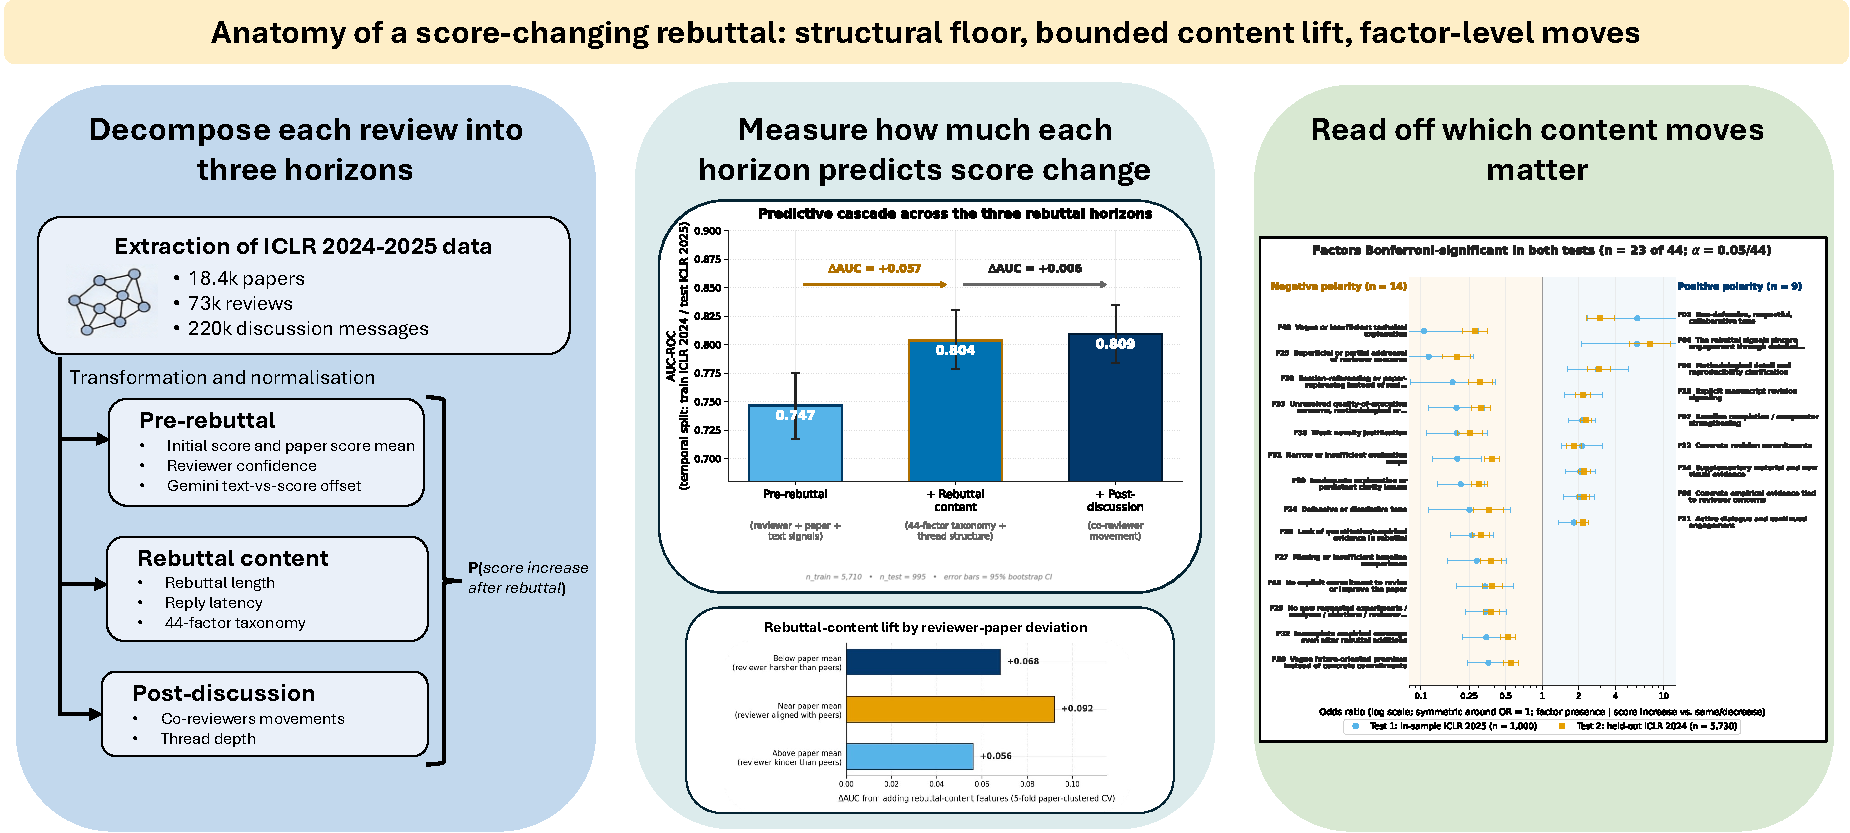
\includegraphics[width=\linewidth]{HeroFigure_V2.pdf}
  \caption{\textbf{Anatomy of a score-changing rebuttal.} (A)~\num{73000} ICLR 2024--2025 reviews split into pre-rebuttal, rebuttal-content (44-factor taxonomy), and post-discussion features predicting whether the reviewer's score rose. (B)~Pre-rebuttal $\auc = 0.747$; rebuttal content adds $+0.057$, post-discussion $+0.006$; lift peaks near the paper mean ($+0.092$). (C)~23 of 44 factors cross Bonferroni in both validation tests (14 negative, 9 positive; 95\% cluster-robust CIs).}
  \label{fig:overview}
\end{figure}

% Section heads in V3 are rewritten as questions. Bodies in this
% scaffold cite which v2 section to migrate. After the scaffold
% compiles, copy the v2 body into each subsection and edit the
% opening sentence to match the question framing.

% ----------------------------------------------------------------------
% 3.1  What rebuttal moves do successful authors actually make?
% ----------------------------------------------------------------------
\subsection{Rebuttals contain 44 distinct content moves, of which 23 robustly track score change}\label{res:taxonomy}

% Migrate from main_v2.tex Section 3.2 (res:taxonomy,
% lines ~337-401). Keep: taxonomy induction with Claude, cross-model
% validation with Gemini, cross-year held-out ICLR 2024 cohort,
% Bonferroni vs BH counts (23 vs 31 of 44), declared polarity. Drop
% the "structural rather than rhetorical" framing here --- save for
% Section 3.3 on conditional associations.
%
% Opening sentence (V3 framing):
%   "To ask which rebuttal moves successful authors make, we induce a
%   content-level taxonomy directly from rebuttal text rather than
%   imposing a prior list of categories."
%
% Why first: V3 prioritises the author-controllable findings.

We induce the taxonomy directly from rebuttal text, rather than imposing a prior list of categories. To do so, we treat each \emph{interaction}, defined as the concatenation of the original review, the author rebuttal, and any reviewer follow-up, as the unit of analysis. Claude Opus 4.6 (LLM-A) sees \num{1000} ICLR 2025 interactions in this raw form, stratified into six cells of initial-score tier crossed with rebuttal outcome (\emph{increase} or \emph{same\_decrease}), and performs a within-tier contrastive analysis. To attenuate run-to-run variability, we repeat the procedure five times and aggregate across runs, yielding 44 factors each with a declared polarity (positive or negative).

A natural worry is that LLM-A is retrieving canonical ``good rebuttal'' patterns from its prior rather than extracting them from the text in front of it. To rule that out, we rerun the induction under two memory-control manipulations on the same \num{1000} interactions: a tier swap, and a silent swap of outcome labels. In both cases the factor content tracks the input data rather than the presented labels (\Cref{app:rebuttal-coding}), so the taxonomy is extracted from the text rather than retrieved from the model's prior.

We then validate the taxonomy with a second, independent model. Gemini Flash 3 (LLM-B) classifies each interaction against the fixed list under an outcome-blinded protocol with shuffled factor identifiers. For every factor we compute an odds ratio with 95\% cluster-robust CI by paper, plus a two-sided permutation test with 2000 permutations. Significance is reported at two thresholds: Bonferroni at $\alpha = 0.05/44 = 0.0011$ as the recommendation gate, and Benjamini-Hochberg at $q = 0.05$ as a sensitivity for the broader taxonomy. The classifier then runs on two cohorts. Test 1 (operationalisability) reuses the \num{1000} ICLR 2025 induction interactions and asks whether an independent model can recover the same factors from the same text. Test 2 (discriminative validity) applies the same protocol to the full ICLR 2024 cohort of \num{5730} interactions, disjoint from the induction corpus, and asks whether the factor--outcome associations replicate on data the taxonomy was never fitted on.

Both tests preserve the declared polarities almost completely: 43 of 44 in Test 1, and all 44 in Test 2. Twenty-three factors cross Bonferroni in both tests (9 positive, 14 negative) and form the conservative core of the taxonomy. Under BH $q = 0.05$ the doubly-significant set grows to 31 of 44, with the eight extras entering the recommendation list as weaker evidence. On the positive side, the doubly-Bonferroni factors include sincere engagement, baseline completion, methodological detail, concrete empirical evidence, and active dialogue. On the negative side, they include defensive or dismissive tone, superficial concern addressal, weak novelty justification, missing baseline comparisons, vague future-oriented promises, and section-referencing in place of clarification.

\begin{figure}[!t]
  \centering
  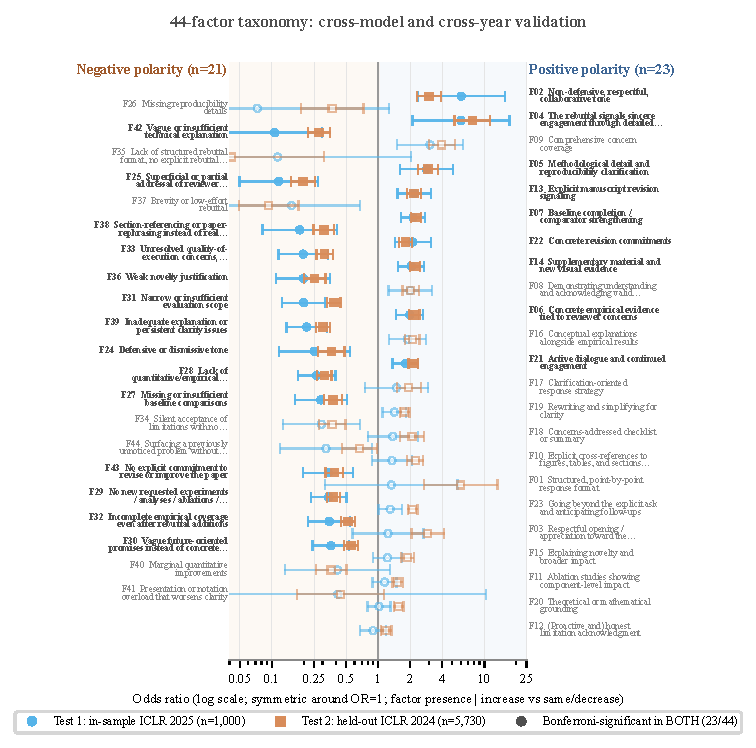
\includegraphics[width=\linewidth]{factor_validation_forest.pdf}
  \caption{\textbf{Cross-model and cross-year validation of the 44-factor taxonomy.} Diverging forest plot on a log-OR axis symmetric around $\text{OR}=1$. Each row shows Test 1 (in-sample ICLR 2025, $n=\num{1000}$, blue circles) and Test 2 (held-out ICLR 2024, $n=\num{5730}$, orange squares); CI caps mark interval endpoints. Filled markers and bold labels highlight the 23 factors that cross Bonferroni in both tests.}
  \label{fig:f3-categories}
\end{figure}

% ----------------------------------------------------------------------
% 3.2  What can the LLM-decoded text-vs-score offset tell us about
%      which reviewers are open to changing their score?
% ----------------------------------------------------------------------
\subsection{Reviewers' initial text already telegraphs whether their score will move}\label{res:instrument}

% Migrate from main_v2.tex Section 3.1 (res:instrument, lines ~264-336).
% Keep: instrument-validation funnel (8/19/32), instrument-calibration
% framing (moderate at agreeing, informative at extracting residual),
% three caveats (LLM-detected, predictive not causal, modest marginal
% contribution after paper-mean control). Discuss the holding-back
% hypothesis as ONE of several plausible mechanisms in Discussion.
%
% Opening sentence (V3 framing):
%   "Once we know what authors might write, we ask which reviewers are
%   most open to revising. Gemini Flash 3 decodes a numeric score from
%   score-stripped review text; the gap between the LLM-decoded score
%   and the reviewer's assigned score is a within-review residual that
%   itself predicts post-rebuttal score movement."

To get at reviewer movability, we use Gemini Flash 3 (\code{gemini-3-flash-preview}) as a score decoder on the initial review text. Before sending each review, we strip every numeric field the reviewer fills in (\code{soundness}, \code{presentation}, \code{contribution}, \code{rating}, \code{recommendation}, and the self-reported \code{confidence} on the 1--5 scale), so the answer cannot leak into the input (\Cref{app:gemini-pred}). Gemini then predicts the score that the remaining text alone implies, and the gap between this decoded score and the reviewer's actually-assigned score is what we call the \emph{text-vs-score offset}. We measure the gap in step positions on the six-point ICLR ladder $\{1, 3, 5, 6, 8, 10\}$ rather than raw points, so adjacent rating pairs all count equally.

Across \num{73000} reviews, Gemini's predictions span the full ICLR scale and roughly track the assigned-score distribution, so the model is not collapsed onto a single value. The decoded score matches the assigned score in $40.7\%$ of reviews, and in the remaining $59.3\%$ Gemini reads the text below the assigned score ($24.3\%$) or above it ($35.0\%$), with mean offset $+0.14$ steps and SD $1.02$. Rank-order correlation is also moderate ($\rho = 0.40$). Taken together, these numbers characterise the instrument as moderate at agreeing with the reviewer but informative at extracting a per-review residual. What our downstream analyses require is not agreement but informative disagreement, which a constant-mode predictor of the score cannot produce.

The crucial test, however, is whether the offset itself predicts later movement, and it does (\Cref{fig:f2-instrument}). Post-rebuttal score-increase rates rise monotonically along the offset, from $8.3\%$ when the LLM reads the text below the assigned score, to $19.2\%$ at agreement, to $31.9\%$ above. The gradient replicates in both years, and a mirror gradient runs for the rarer post-rebuttal decreases ($3.3\%$ under, $1.0\%$ at zero, $0.4\%$ over, against a $1.4\%$ baseline overall). Put together, under-offset reviewers are about eight times more likely to revise down than over-offset reviewers, and over-offset reviewers about four times more likely to revise up. To check that this signal is not merely a shadow of the auxiliary per-review ratings Gemini also produces (engagement, sentiment, tone), we add all three jointly as covariates in a logistic model. The offset coefficient shrinks by $23.6\%$ (from $0.643$ to $0.492$, \Cref{app:text-score-gap}), so about three-quarters of its predictive power sits outside these alternative ratings.

These results carry several caveats. The label ``LLM-detected'' does real work, since there is no non-LLM gold standard for what review text should imply. The relationship is predictive rather than causal, and the offset's marginal contribution shrinks further once paper-mean position is controlled (\Cref{sec:horizons}). Several mechanisms are consistent with the funnel, and we return to them in \Cref{sec:discussion}.

\begin{figure}[!htb]
  \centering
  \begin{subfigure}[b]{0.49\linewidth}
    \centering
    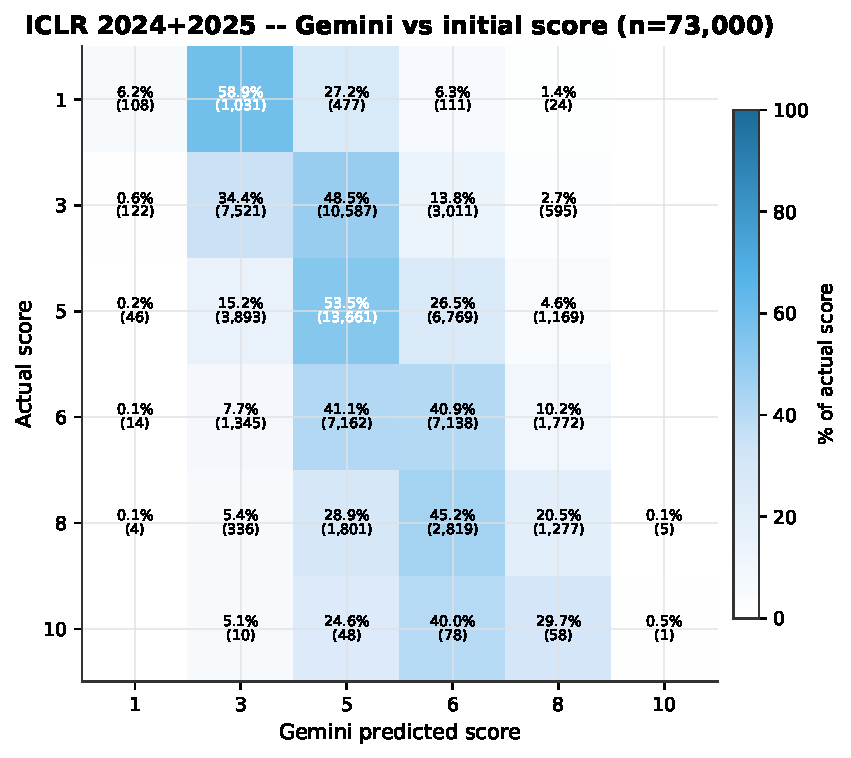
\includegraphics[width=\linewidth]{gemini_pred_combined_confusion_initial.pdf}
    \caption{Score-decoding accuracy}
    \label{fig:f2-confusion}
  \end{subfigure}\hfill
  \begin{subfigure}[b]{0.49\linewidth}
    \centering
    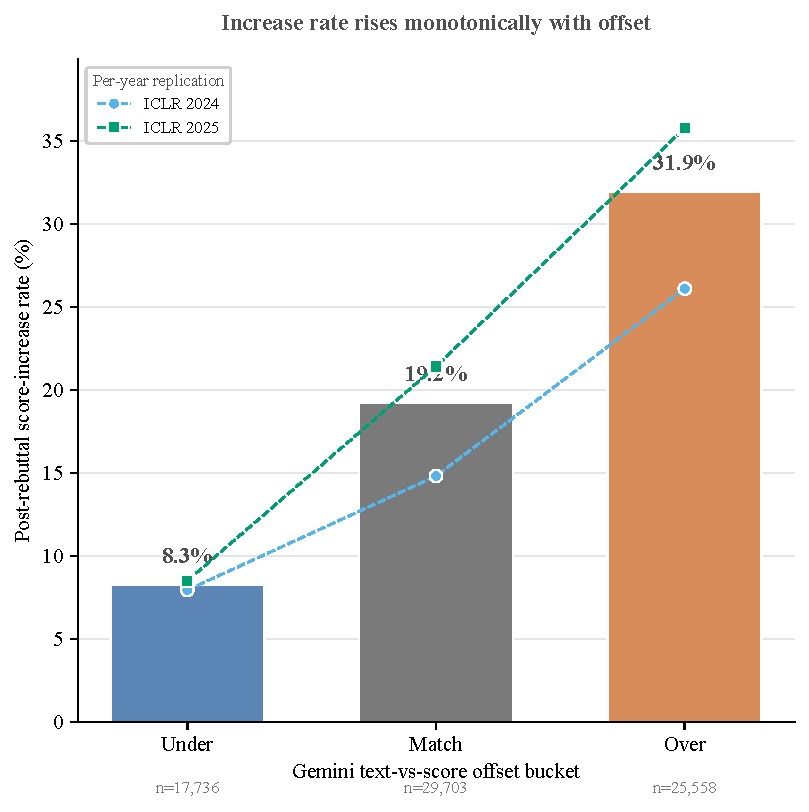
\includegraphics[width=\linewidth]{funnel_increase_rate.pdf}
    \caption{Text-vs-score-gap funnel}
    \label{fig:f2-funnel}
  \end{subfigure}
  \caption{\textbf{Gemini Flash 3 as instrument: score decoding and the within-review calibration signal.} (\subref{fig:f2-confusion}) Row-normalised confusion matrix of Gemini-decoded vs.\ external pre-rebuttal scores on the combined ICLR 2024+2025 cohort ($n=\num{73000}$). (\subref{fig:f2-funnel}) Post-rebuttal score-increase rate by Gemini text-vs-score offset bucket; combined bars and per-year markers (numbers in \Cref{res:instrument}).}
  \label{fig:f2-instrument}
\end{figure}

% ----------------------------------------------------------------------
% 3.3  Which moves are independently associated with success after
%      controlling for who's reviewing?
% ----------------------------------------------------------------------
\subsection{Content moves dominate, and tone matters at the margins}\label{sec:horizons}

% Migrate from main_v2.tex Section 3.3 (sec:horizons, lines ~403-411
% prose, plus app:horizons coefficient table).
% Keep: paper-clustered logistic, asymmetric polarity screen (4
% positive + 10 negative), Bonferroni and BH reporting, structural
% confounders dwarfing per-factor associations, no-pos_before
% ablation result (movability envelope holds, RF AUC drops 0.001-0.011),
% null-triplet defense (rebuttal length, n_replies flatly null with
% MDE >= 1.20; first-reply latency borderline at OR=0.90, p=0.12).
%
% Opening sentence (V3 framing):
%   "Section 3.1 produced a list of 44 factors with declared polarities.
%   We now ask which of those associations survive once we control for
%   who is reviewing, which paper they are reviewing, and how the paper
%   looks at initial-review time. The answer governs which factors
%   appear on a recommendation list authors might consult."

We now ask which of the 44 factors remain associated with score increase once we control for who is reviewing and what the paper looks like at initial-review time. We fit a paper-clustered logistic regression on the combined 2024+2025 rebuttal cohort ($n = 6{,}705$, base rate $45.6\%$), regressing score-increase on the 44 factor indicators alongside ten structural confounders and four rebuttal-side aggregates that track prior structural-correlate analyses~\cite{huang,jung,kargaran}. The full feature catalogue, the leakage audit, and the asymmetric screen rules sit in \Cref{app:horizons}.

Before reading off the per-factor effects, we have to handle one structural feature of the rebuttal-content space. Positive and negative factors tend to be anti-correlated within a rebuttal: a draft that does baseline completion rarely also does superficial concern addressal, so the two polarity blocks compete for variance in a single joint fit and crowd the positive coefficients toward zero. We therefore screen positives and negatives separately, accepting a factor as robustly associated with score increase only if it survives both a univariate marginal screen and a polarity-isolated joint screen, with both 95\% CIs excluding $1$. Under this asymmetric screen, four of the 22 testable taxonomy positives (after dropping near-constant $F_{01}$) and ten of the 18 testable taxonomy negatives (after dropping three rare negatives at $<1\%$ prevalence) qualify (\Cref{fig:recforest}). On the positive side, the strongest are $F_{07}$ baseline completion (OR $= 1.64$ [$1.42$, $1.89$], the only positive to clear Bonferroni in the headline joint), followed by $F_{02}$ non-defensive tone ($1.51$), $F_{19}$ writing fixes ($1.27$), and $F_{20}$ theoretical grounding ($1.18$). On the negative side, $F_{39}$ inadequate or persistently unclear explanation (OR $= 0.31$ [$0.25$, $0.39$]) and $F_{37}$ brevity or low-effort rebuttal ($0.38$) lead, followed by $F_{24}$ defensive or dismissive tone, $F_{36}$ weak novelty justification, and several others, and seven of the ten qualifying negatives clear Bonferroni in the headline joint as well. As a one-number summary of polarity, a binomial sign test on the declared direction rejects chance at $p = 0.026$ on the positives and $p = 0.0038$ on the negatives.

The structural confounders, in contrast, dwarf the per-factor associations, as expected. Within them, initial-score position is the single largest contributor (per 1 SD, OR $= 0.141$ [$0.122$, $0.163$]: high initial scores cannot rise), followed by paper-level initial mean (OR $= 1.89$) and the \code{contribution} sub-score (OR $= 1.70$). Even after the 44 factors are controlled, the Gemini text-vs-score offset of \Cref{res:instrument} still survives at OR $= 1.15$ [$1.06$, $1.26$]. Among the rebuttal-side aggregates, two clear conventional significance: maximum thread depth (OR $= 1.24$, Bonferroni-significant) and days remaining until the review-submission deadline (per 1 SD $\approx 4.7$ days, OR $= 1.19$, $p = 0.011$).

Three other rebuttal-side features come out flat in the joint specification. Rebuttal length and the number of author replies sit at per-SD ORs of $1.02$ and $0.95$ ($p > 0.4$), and first-reply latency trends toward a small negative effect (per 1 SD OR $= 0.90$, $p = 0.12$) without clearing significance. The flatness is not just a power problem: with $80\%$ power against per-SD ORs $\geq 1.20$ in this design (\Cref{app:horizons}), the nulls rule out moderate effects but not small ones. The Gemini engagement rating tells a similar story. On its own it predicts increase well (OR per SD $= 1.30$, $p < 10^{-4}$), but the effect disappears once the 44 factors are in the model (OR $= 1.04$, $p = 0.44$). The 44 factor indicators absorb essentially all of the engagement-rating variance that predicts score increase.

Stepping back, the single largest predictor of post-rebuttal increase is structural rather than rhetorical. A reviewer who scored a paper below its initial co-reviewer mean has more headroom and more social pressure to revise upward than one who already scored at or above the mean. The structural envelope is not localised to the explicit \code{pos\_before} column alone: it still holds when we drop \code{pos\_before} from the feature set, with the magnitudes reported in \Cref{sec:rebuttal-impact}. We caveat this ablation. \code{paper\_initial\_mean} and \code{deviation\_from\_paper\_mean} together linearly reconstruct \code{pos\_before}, so the residual signal after removing only \code{pos\_before} continues to leak the focal score through the remaining features. The ablation therefore shows that the model does not depend on \code{pos\_before} being named explicitly, not that the prediction is independent of the focal score. A stricter ablation that drops all three would mechanically remove the within-review score information and is reserved as future work.

Stratification makes the same point in a different way. Refitting the headline logistic on three strata defined by deviation from the paper-level initial mean confirms a threefold base-rate gradient: below paper mean ($n = 2{,}602$, $62.8\%$ base rate), near paper mean ($n = 2{,}302$, $46.0\%$), and above paper mean ($n = 1{,}801$, $20.2\%$). Rebuttal-content effects survive within each stratum, and $F_{07}$ and $F_{39}$ keep their direction in all three (\Cref{fig:movability-strata}). Predictive performance is also heterogeneous across these strata, with the heaviest rebuttal-content lift among reviewers near the paper mean. The per-stratum AUC numbers sit in \Cref{sec:rebuttal-impact}. As throughout, the language is correlational: a factor's odds ratio summarises the empirical association, not a causal claim about intentionally inserting the factor into a draft.

\begin{figure}[!htb]
  \centering
  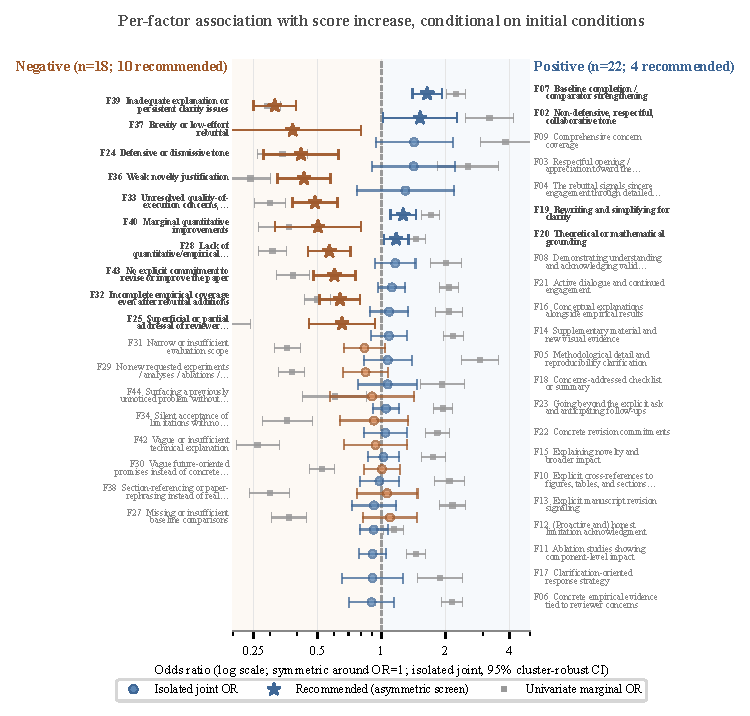
\includegraphics[width=\linewidth]{forest_recommendation.pdf}
  \caption{\textbf{Per-factor association with score increase, conditional on initial conditions.} Diverging forest plot: positive-polarity factors on the right (blue), negative-polarity factors on the left (orange), sharing one log-OR axis symmetric around $\text{OR}=1$. Each row shows the polarity-isolated conditional OR (large marker) and the univariate marginal OR (small grey square), with CI caps marking interval endpoints. $\star$ marks the 14 factors that pass the asymmetric screen (4 of 22 testable positives, 10 of 18 testable negatives; screen definition in \Cref{sec:horizons,app:horizons}). Negatives sit at half-row offsets so the two polarities interleave; same-row pairings reflect within-polarity rank only.}
  \label{fig:recforest}
\end{figure}

\begin{figure}[!htb]
  \centering
  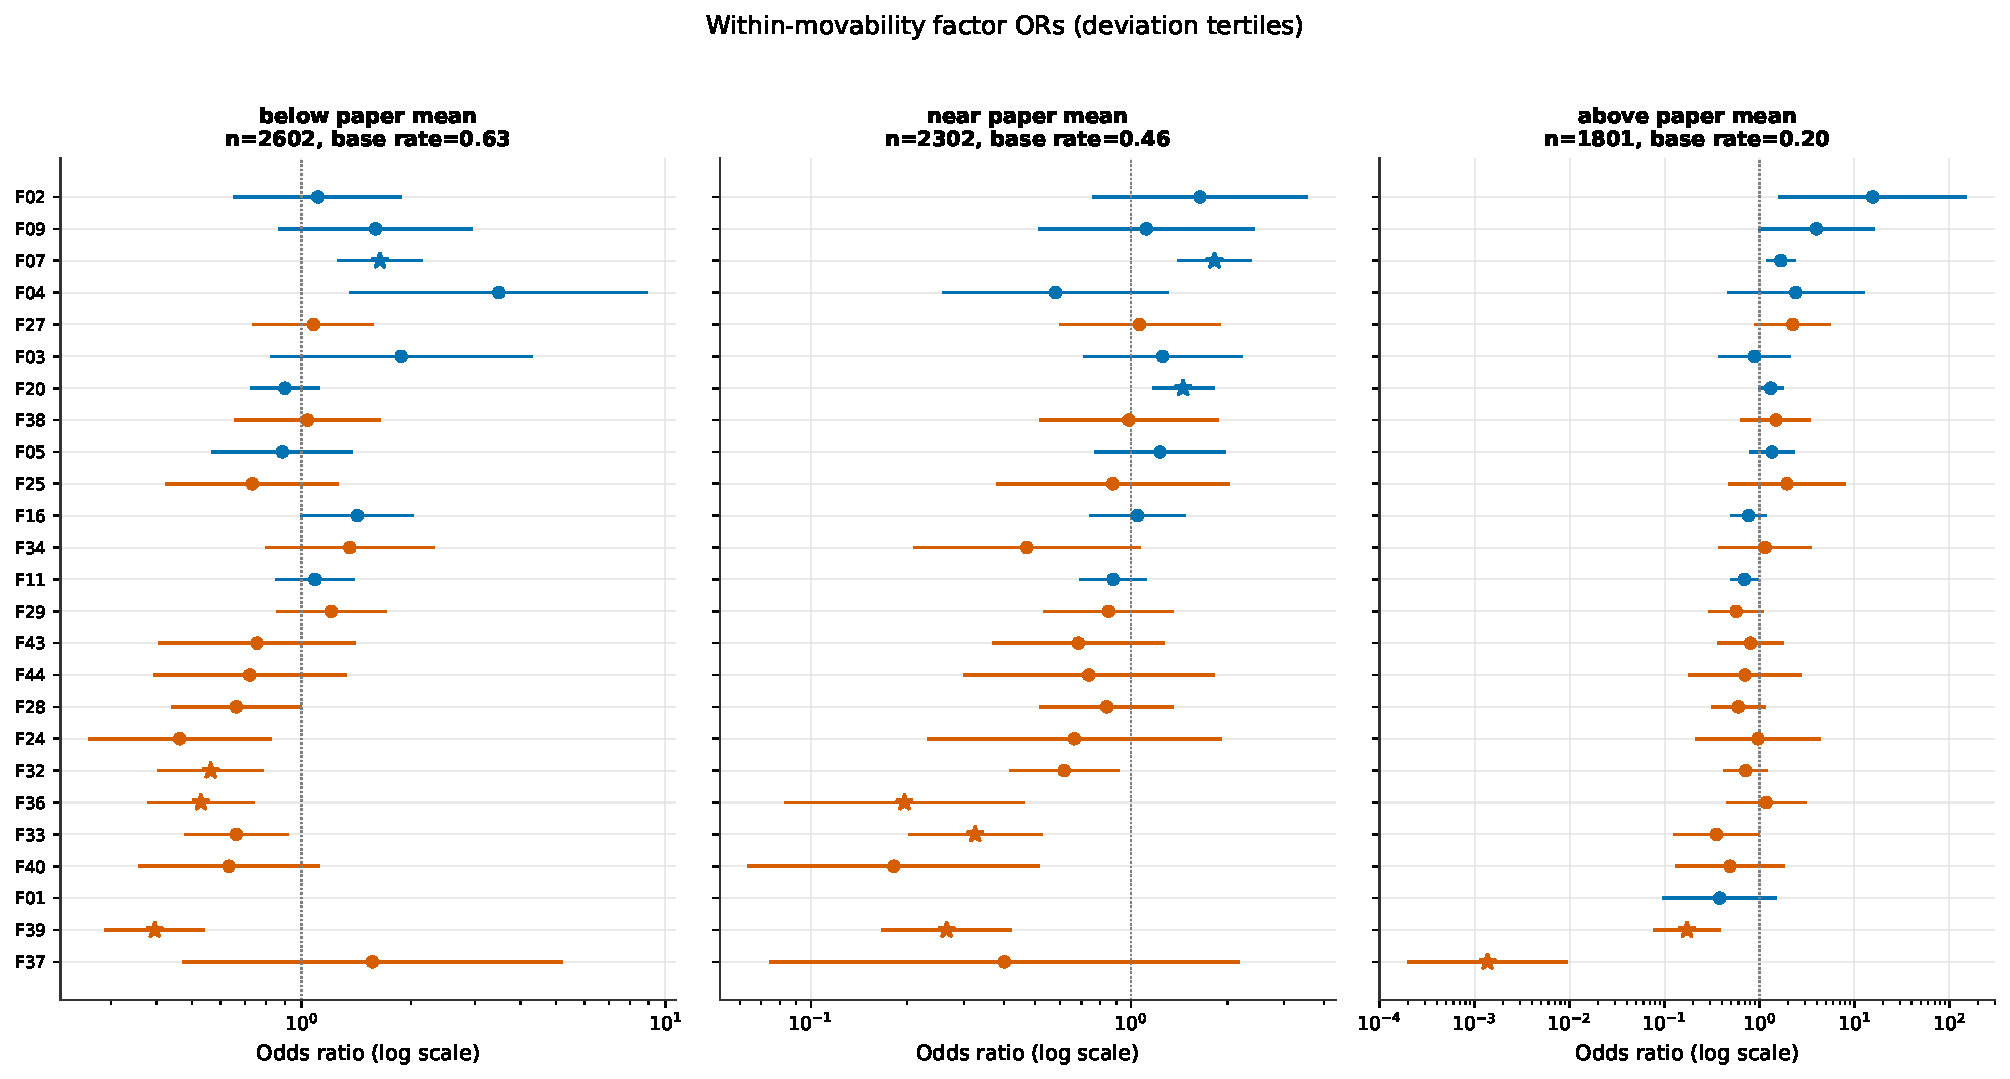
\includegraphics[width=0.7\linewidth]{forest_movability_strata.pdf}
  \caption{\textbf{Per-factor odds ratios within reviewer-paper movability strata.} Forest plot for the 44 factors fit separately within three strata defined by reviewer deviation from the paper-level initial mean: below ($n=2{,}602$, $62.8\%$ base rate), near ($n=2{,}302$, $46.0\%$), above ($n=1{,}801$, $20.2\%$). Qualifying factors keep their declared direction in all three strata; per-stratum AUC lifts in \Cref{sec:rebuttal-impact}.}
  \label{fig:movability-strata}
\end{figure}

% ----------------------------------------------------------------------
% 3.4  How much of the outcome is movable, and at which authoring
%      stage?
% ----------------------------------------------------------------------
\subsection{Most recoverable predictive signal is present before rebuttal, but content still adds a bounded $+0.057$ AUC}\label{sec:rebuttal-impact}

% Migrate from main_v2.tex Section 3.4 (sec:rebuttal-impact, lines
% ~502-547). Keep: temporal split AUC cascade 0.744 -> 0.801 -> 0.806,
% within-strata heterogeneity (+0.092 / +0.068 / +0.056), Table 1
% scenarios under the V2 reframing (with X present, not + add X), and
% the per-stratum recommendation set.
%
% Opening sentence (V3 framing):
%   "The previous sections quantified within-review signal and
%   within-rebuttal content signal separately. We now ask what fraction
%   of the post-rebuttal score-increase outcome is movable at each
%   observable stage: pre-rebuttal (when only structural conditions are
%   visible), rebuttal-content (when the resolved rebuttal thread is
%   present), and post-discussion (when co-reviewer movement is
%   observable). We label the middle horizon `rebuttal-content' rather
%   than `draft-time' because the factor classifier reads the full
%   resolved thread, including reviewer follow-ups, so the indicators
%   are properties of the resolved interaction rather than cleanly
%   author-controllable draft features."

We now ask how much of the score-change outcome is recoverable at all, and at which authoring stage. The outcome is a binary indicator at the (paper, reviewer) level: $\code{score\_increase} = 1$ if the reviewer's post-rebuttal rating is strictly greater than their pre-rebuttal rating, and $0$ otherwise. The cohort is restricted to reviews that received at least one author reply, since horizons that contain rebuttal-content features are undefined when no rebuttal exists. This cohort skews above the no-rebuttal subset on initial score (mean $5.1$ vs $4.0$) and on deviation from paper mean ($+0.10$ vs $-0.32$), so the pre-rebuttal $\auc$ reported below should be read as predictability within reviews where the author chose to engage, rather than as a population-level floor. We slice the same rebuttal-content logistic three ways: by horizon, by out-of-time calibration, and by scenario sensitivities for a representative author. The full feature catalogue at each horizon, the evaluation protocol (temporal split and paper-clustered $\texttt{GroupKFold}(5)$), and the leakage audit sit in \Cref{app:horizons}. All AUC and AUPRC numbers below refer to predicting this binary outcome. We deliberately label the middle horizon \emph{rebuttal-content} rather than \emph{draft-time}. The factor classifier reads the full resolved thread, including reviewer follow-ups, so the indicators are properties of the resolved interaction rather than cleanly author-controllable draft features.

We start with the pre-rebuttal horizon. The block uses only what is visible before the author writes a word: structural confounders, review-text features, and the Gemini text-derived signals of \Cref{res:instrument}. Even with no rebuttal information at all, it already reaches $\auc = 0.747$ [$0.72$, $0.77$] and $\auprc = 0.724$ [$0.68$, $0.76$] for predicting score increase on the temporal test (\Cref{fig:horizons}). Most of this pre-rebuttal floor comes from a small set of features: the focal reviewer's deviation from the paper's initial mean, their initial-score position, and the text-vs-score offset. One natural worry is that this floor is a mechanical artefact of the focal score itself, since \code{pos\_before} constrains the direction of movement. Refitting the pre-rebuttal block without \code{pos\_before} reaches temporal-split AUC $0.724$ (RF) and $0.718$ (logistic), losing only $\Delta\auc = -0.001$ to $-0.029$ against the full block. This says the pre-rebuttal predictability is not localised to the named \code{pos\_before} column. It does not say the prediction is independent of the focal score, because \code{paper\_initial\_mean} and \code{deviation\_from\_paper\_mean} together still reconstruct \code{pos\_before} linearly. The ablation isolates linear redundancy across the score-derived features rather than testing independence from the score itself, and a stricter ablation that drops all three score-derived features would mechanically remove the within-review score information.

Adding the rebuttal-text aggregates and the 44 factor indicators then lifts both metrics to $\auc = 0.804$ [$0.78$, $0.83$] and $\auprc = 0.780$ [$0.75$, $0.81$]. The temporal gain is $\Delta\auc = +0.057$ and $\Delta\auprc = +0.056$, and it replicates under cross-validation at $\Delta\auc = +0.069$. The two metrics agree at the cohort's base rate of $44.4\%$. Adding co-reviewer movement and thread-depth aggregates at the post-discussion horizon adds little on top ($\Delta\auc = +0.006$ on the temporal split, $+0.010$ in cross-validation), as expected for a horizon whose features sit downstream of the rebuttal we are trying to predict. Most of the recoverable signal is therefore set before the author writes anything, and the rebuttal adds a real but bounded $+0.06$ to $+0.07$ AUC inside that envelope. A random forest on the same features at every horizon never exceeds the logistic by more than $0.01$ AUC, so the linear model already reaches the predictive ceiling these features can support. Within the three movability strata of \Cref{sec:horizons}, the lift is $+0.068$ AUC below the paper mean, $+0.092$ near the mean, and $+0.056$ above (5-fold paper-clustered CV), so reviewers near the mean see the heaviest gain even though those below the mean carry most of the absolute movement budget.

\begin{figure}[!htb]
  \centering
  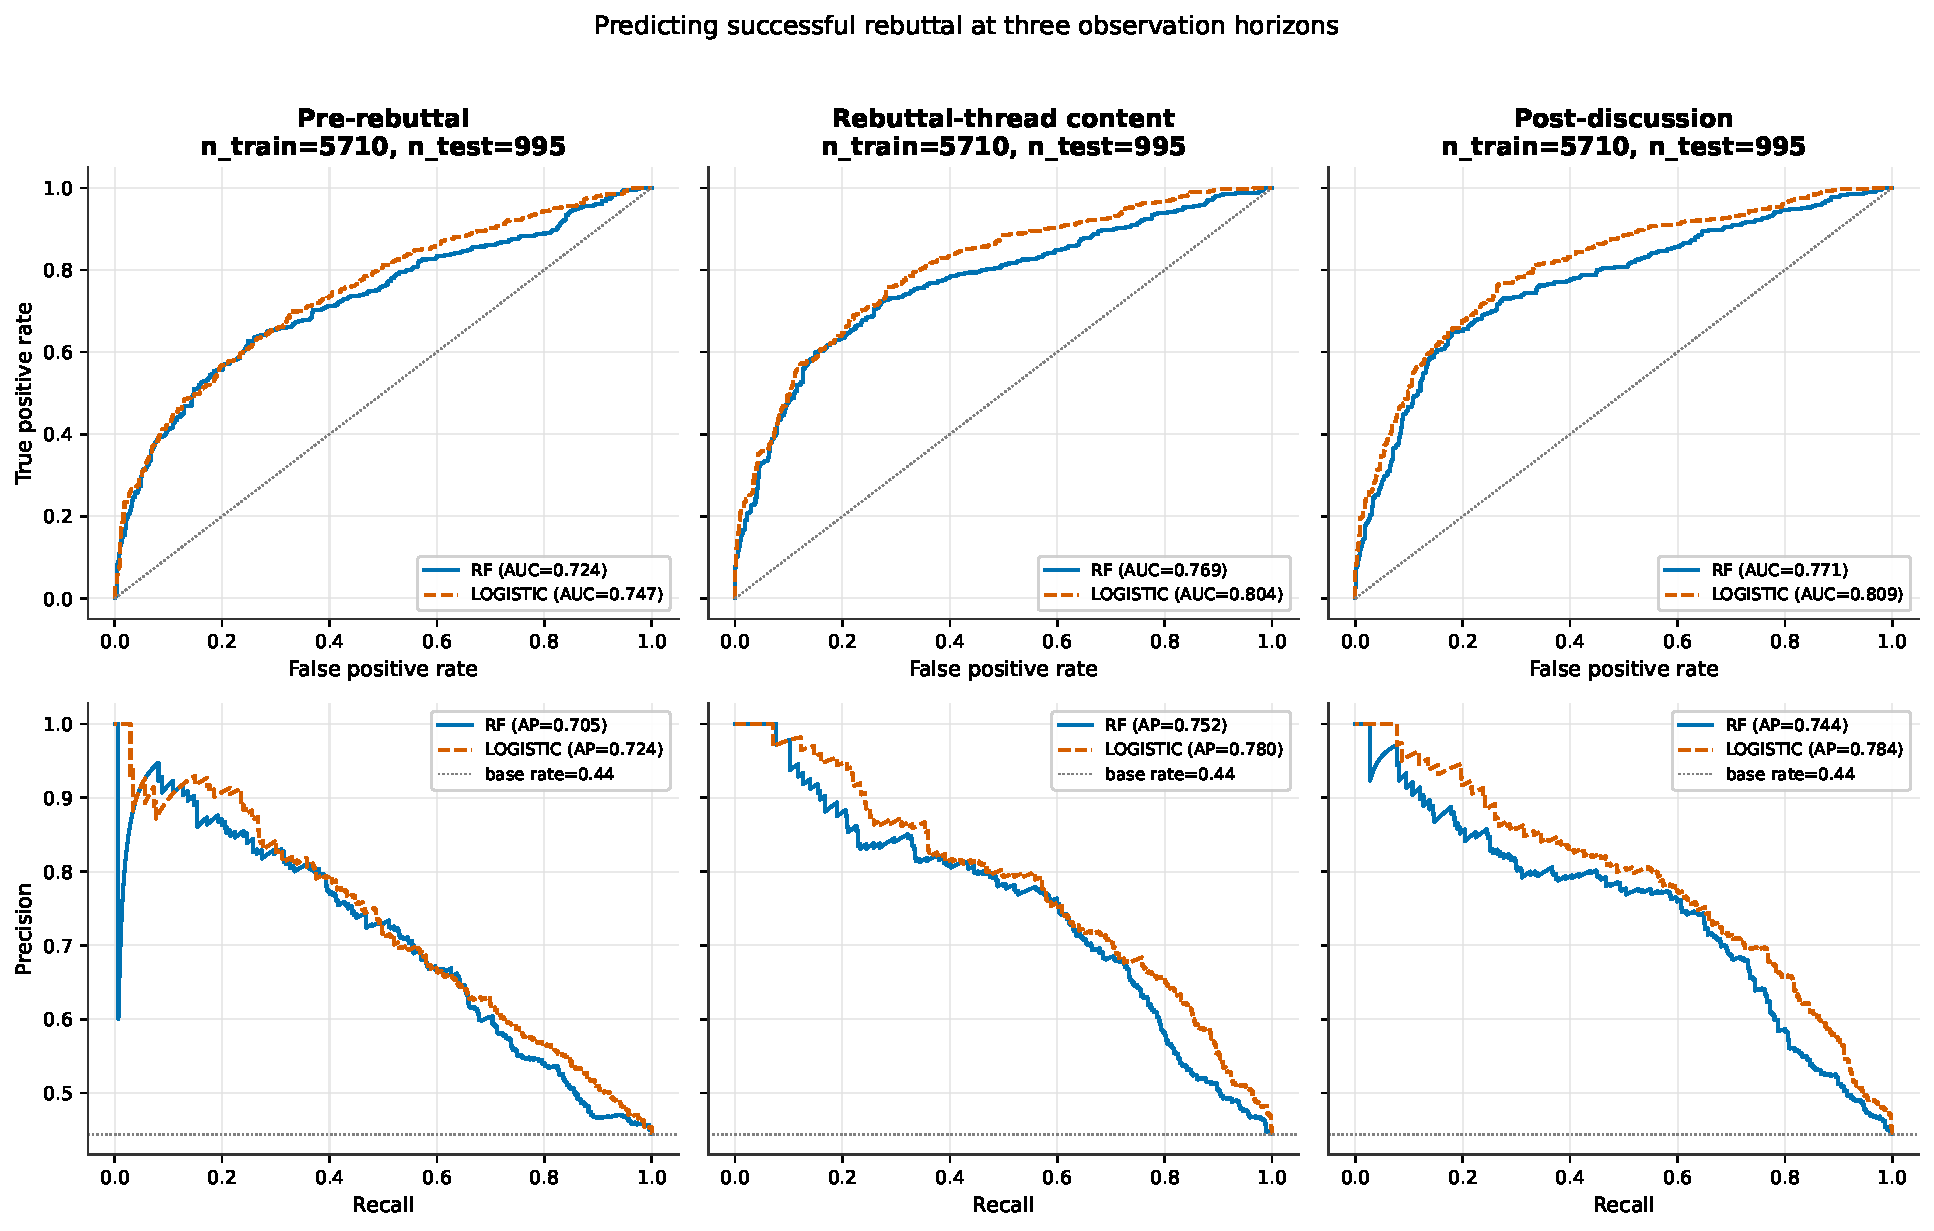
\includegraphics[width=0.7\linewidth]{figure_horizons.pdf}
  \caption{\textbf{Cascade of predictive performance across observation horizons.} ROC (top) and precision-recall (bottom) curves for random forest (solid blue) and L2-regularised logistic (dashed orange) on the temporal split (train ICLR 2024, $n=5{,}710$; test ICLR 2025, $n=995$). AUC values per horizon and the $\Delta\auc$ between them are reported in \Cref{sec:rebuttal-impact}.}
  \label{fig:horizons}
\end{figure}

Out-of-time calibration (full plot in \Cref{app:horizons}) is reliable at the extremes but loose in the middle. The top decile predicts $0.94$ against an observed $0.89$, the bottom decile predicts $0.05$ against an observed $0.14$, and two middle deciles over-predict by up to $0.16$. So while the rank ordering carries the load across the full range, the absolute probability scale is trustworthy mainly at the extremes, and a fixed-threshold readout would under-use the information the model carries.

To put the lever in author-facing terms, we hold a 2024-median author profile fixed (median initial score, median paper mean, neutral confidence, neutral Gemini offset) and read off the model's predicted probability of score increase under several rebuttal configurations. Without any qualifying factors present, the probability sits at $0.22$. It rises to $0.32$ for a rebuttal with $F_{07}$ baseline completion present, $0.47$ with the top-3 qualifying positives ($F_{07}$, $F_{02}$, $F_{19}$), and $0.53$ with all four qualifying positives ($F_{07}$, $F_{02}$, $F_{19}$, $F_{20}$) (\Cref{tab:scenarios}). On the negative side, a rebuttal that exhibits the top-3 qualifying negatives ($F_{39}$, $F_{37}$, $F_{24}$) alongside all four qualifying positives sits at $0.09$, and one that exhibits only the negatives sits at $0.02$. The asymmetry is informative: rebuttals without the top qualifying negatives carry predicted probabilities comparable to rebuttals with the top qualifying positives. These numbers are conditional probabilities under the observational model, not interventional estimates. An interventional version would require randomised assignment of factor inclusion across rebuttals, which our design cannot deliver. With those caveats, the magnitudes give a sense of the incremental predictive lift from rebuttal-thread content associated with each configuration.

\begin{table}[!htbp]
  \centering
  \caption{Predicted score-increase probability under the rebuttal-content logistic for a 2024-median author profile whose rebuttal already exhibits the listed factors. The numbers are conditional probabilities under the observational model, not interventional estimates. ``Top-$k$ qualifying'' refers to the $k$ factors with the largest isolated odds ratio in the declared direction among those that meet the asymmetric association screen (\Cref{fig:recforest}). Probabilities read off the same rebuttal-content logistic used in \Cref{sec:horizons}.}
  \label{tab:scenarios}
  \small
  \begin{tabular}{lr}
    \toprule
    Rebuttal configuration (factors observed to be present) & $P(\text{score increase})$ \\
    \midrule
    Median author profile, no qualifying factors                                       & $0.22$ \\
    With $F_{07}$ baseline completion present                                          & $0.32$ \\
    With the top-3 qualifying positive factors present                                 & $0.47$ \\
    With all four qualifying positive factors present                                  & $0.53$ \\
    With all four positives \emph{and} top-3 negatives present                         & $0.09$ \\
    With top-3 qualifying negative factors only (no positives)                         & $0.02$ \\
    \bottomrule
  \end{tabular}
\end{table}

Together, the 44-factor classifier, the Gemini score decoder, and the rebuttal-content logistic map a resolved rebuttal interaction plus the publicly visible reviewer and paper metadata to a predicted probability of score increase. The qualifying-factor list and the scenario sensitivities are our actionable contribution: an association screen over the moves most tied to score change, with an order-of-magnitude sense of how their presence shifts the predicted probability for a representative author. Reading the screen as an interventional recipe is not warranted by the evidence.

% ======================================================================
% 4. DISCUSSION  (V3 reframe: calibrated three-sentence message)
% ======================================================================
\section{Discussion}\label{sec:discussion}

% V3 Discussion structure:
%   - Calibrated three-sentence headline takeaway (replaces the v2
%     "Synthesis" paragraph).
%   - Why the LLM-text signal is bounded (keep largely as-is from v2).
%   - Plausible mechanisms for the offset signal (FLOAT the
%     holding-back hypothesis as ONE of several, alongside reviewer
%     headroom, reviewer calibration, and the LLM's own score prior).
%   - What this means for authors (three sentences, calibrated).
%   - What this means for venues (one sentence on the rebuttal
%     mechanism resolving a measurable share of score-disagreement
%     noise).
%   - Limitations (carry forward v2 Limitations including Thakkar
%     contamination, full-thread factor extraction, no human gold
%     standard for the taxonomy).
%   - Future work (cross-venue replication, prospective intervention
%     studies, draft-only re-classification).

\paragraph{Calibrated takeaway.}
The three findings fit together. First, the pre-rebuttal $\auc$ of $0.747$ tells us that most of the recoverable predictive signal is already present before the author writes a word, dominated by the focal reviewer's initial score and the paper-level initial mean. Note that AUC measures rank-ordering of the binary score-increase outcome, not causal movability, so this number bounds what is recoverable from observable features rather than what is structurally fixed. The rebuttal then adds a real but bounded lever ($+0.057$ AUC), and that lever is largest for reviewers near the paper mean ($+0.092$). Within that lever, an asymmetric polarity screen picks out a small set of content moves (baseline completion, non-defensive tone, writing fixes, theoretical grounding) that are robustly associated with score increase across years and within movability strata. All three are associations in observed interactions rather than interventions.

\paragraph{Without a rebuttal, scores rarely move.} Our predictive cohort conditions on reviews that received at least one author reply ($n=6{,}705$ factor-labeled, base rate $44.4\%$). Across the broader externally-ground-truthed corpus (\num{73231} matched reviews, abbreviated to \num{73000} elsewhere in this paper), reviews where the author never replied ($n=17{,}990$, about a quarter of all reviews) increase only $2.7\%$ of the time, against $27.0\%$ for the with-rebuttal subset. The roughly tenfold gap is observational rather than causal. Authors may skip rebuttals against clear accepts or clear rejects, and reviewers may stop engaging once the verdict feels cemented. The two cohorts are also structurally different. No-rebuttal reviews skew toward lower initial scores (mean $4.0$ vs $5.1$) and below the paper mean (deviation $-0.32$ vs $+0.10$), so the pre-rebuttal $\auc$ reported in \Cref{sec:rebuttal-impact} is best read as predictability among reviews that already passed the rebuttal-engagement filter. The $491$ no-rebuttal reviews whose score nonetheless increased almost always sit on threads with at least one non-author reply ($12.2\%$ of the increased no-rebuttal cases versus $1.4\%$ of the unchanged ones), pointing to area-chair discussion or co-reviewer movement as the most likely vehicle.

\paragraph{What this means for authors.} Most of the reviewer-level score-increase outcome is set before you write a word. The rebuttal lever exists and is largest when your scores are near the paper-level mean. The moves most strongly associated with score increase are baseline completion, non-defensive tone, writing fixes, and theoretical grounding. The moves most strongly associated with no change are inadequate explanation, low-effort rebuttals, defensive tone, and weak novelty justification. These are associations in observed interactions, not interventions: the model summarises the rebuttals authors wrote and does not estimate the causal effect of intentionally inserting a factor into a draft.

\paragraph{Limitations.} The corpus is ICLR 2024 and 2025 only, and the rating scale is ordinal with uneven steps. Both limit cross-venue and cross-time portability. The 2025 factor-validation cohort is a stratified $1{,}000$-pair sample rather than a representative draw, because budgeted access to a paid LLM API constrained how many interactions we could classify with the factor prompt. All statistical language is correlational. We use paper-clustered standard errors, but there is no causal identification, and observed associations may reflect unmeasured paper-level confounds. The rebuttal-content horizon is observationally defined: factor indicators come from the resolved thread, including reviewer follow-ups, so per-factor odds ratios are properties of the resolved interaction rather than guarantees about the author's first-shot draft. Within-rebuttal multicollinearity between positive and negative factors required the asymmetric polarity screen, so individual joint coefficients should be read alongside the marginal and polarity-isolated refits in \Cref{app:horizons}. The 44-factor taxonomy was validated cross-model and cross-year against the externally-archived score outcome but not against a human-coded gold standard. Per-factor labels therefore reflect what two independent LLMs agree to extract from text rather than ground-truth content judgements. Finally, our ICLR 2025 reviews overlap with the randomised LLM-feedback intervention of Thakkar et al.~\cite{thakkar}, in which roughly a quarter of treated reviewers updated their reviews. We did not exclude treatment-arm reviews because the assignment indicators are not public. The randomisation was at the review level, so any effect on our estimates should average out rather than bias them in a known direction. The ICLR 2024 cohort, used as the temporal training year, predates the intervention and is uncontaminated. If treatment indicators become available, the analyses would be straightforwardly recomputable on the untreated subset.

\paragraph{Future work.} The most direct next step is cross-venue replication on NeurIPS, ICML, and less-anonymised conferences, where the base rate of post-rebuttal change and the structural confounders may shift. Beyond that, the gap between association and causation calls for prospective intervention studies that test the recommendation screen against actual draft-level edits. A more focused refinement is to re-run the 44-factor classification on author-only first-shot rebuttal text (excluding reviewer follow-ups). This would isolate author-controllable factors from emergent ones and sharpen the per-factor odds ratios for use in writing guidance.

% ======================================================================
% 5. REFERENCES
% ======================================================================
\bibliography{references}

\appendix

\section{Methods and supplementary materials}\label{app:methods}
% Umbrella section. Each \subsection below is a methodological block
% referenced from the main text. Subsection bodies are placeholders;
% content sources are listed in comments so prose can be drafted in a
% follow-up session by salvaging from main.tex and the docs/methodology/
% files.

\subsection{Dataset}\label{app:dataset}

We collected all publicly visible submissions, reviews, decisions, and discussion data from four years of ICLR (2023--2026) via the OpenReview API on the following dates: ICLR 2023--2024 on November 3, 2025, ICLR 2025 on January 21, 2026, and ICLR 2026 on March 31, 2026. The latest discussion activity recorded is May 2, 2025 for ICLR 2025 and March 28, 2026 for ICLR 2026. Table~\ref{tab:dataset-appendix} provides the per-year composition.

\begin{table}[htbp]
  \centering
  \caption{Extended dataset composition. Message counts reflect individual posts. Engagement rates count distinct participant-paper events. Acceptance rates differ slightly from PaperCopilot for 2023 (footnote $d$) and for 2024--2025 (footnote $e$); for 2026, rates match exactly.}
  \label{tab:dataset-appendix}
  \small
  \begin{tabular}{lrrrrr}
    \toprule
    & \textbf{2023} & \textbf{2024} & \textbf{2025} & \textbf{2026} & \textbf{Total} \\
    \midrule
    Papers (total)                & \num{3793}  & \num{7404}  & \num{11672} & \num{19814} & \num{42683}  \\
    \quad with reviews            & \num{3793}  & \num{7262}  & \num{11520} & \num{19474} & \num{42049}  \\
    \quad without reviews         & 0           & 142         & 152         & 340         & 634          \\
    Reviews                       & \num{14339} & \num{28028} & \num{46748} & \num{75859} & \num{164974} \\
    Reviews per paper             & 3.8         & 3.9         & 4.1         & 3.9         & 3.9          \\
    \midrule
    Discussion messages           & \num{36875} & \num{70624} & \num{149221}& \num{180144}& \num{436864} \\
    \quad Author messages         & \num{30189} & \num{56082} & \num{115034}& \num{159454}& \num{360759} \\
    \quad Reviewer messages       & \num{6376}  & \num{14016} & \num{32938} & \num{19559} & \num{72889}  \\
    \quad AC/PC messages          & 310         & 526         & \num{1235}  & \num{1131}  & \num{3202}   \\
    Author response rate$^a$      & 88.7\%      & 80.1\%      & 74.6\%      & 74.0\%      &              \\
    Reviewer follow-up rate$^b$   & --          & 17.5\%      & 17.7\%      & 12.2\%$^c$  &              \\
    \midrule
    Acceptance rate (ours)        & 41.5\%$^d$  & 30.5\%      & 31.7\%      & 27.0\%      &              \\
    Acceptance rate (PaperCopilot)& 31.8\%      & 31.0\%      & 32.1\%      & 27.0\%      &              \\
    Rating scale                  & \multicolumn{3}{c}{$\{1, 3, 5, 6, 8, 10\}$} & $\{0, 2, 4, 6, 8, 10\}$ & \\
    API version                   & v1          & \multicolumn{3}{c}{v2} &              \\
    \bottomrule
  \end{tabular}
\end{table}

\noindent\footnotesize
$^a$ Fraction of papers with at least one author comment.
$^b$ Fraction of reviews where the reviewer posted at least one follow-up comment. Not available for 2023 (API v1 does not reliably distinguish reviewer follow-ups from initial reviews).
$^c$ ICLR 2026 data was collected March 31, 2026. The low reviewer follow-up rate likely reflects incomplete discussion data, as the latest recorded follow-up is March 28, 2026.
$^d$ Our 2023 acceptance rate (41.5\%) differs from PaperCopilot (31.8\%) because our dataset is missing ${\sim}\num{1162}$ withdrawn or desk-rejected papers (see below). PaperCopilot computes acceptance over all \num{4955} submissions.\\
$^e$ The 0.4 to 0.5 percentage-point gap for 2024 and 2025 likely reflects papers that were accepted and then later withdrawn. We classify these by final OpenReview status (Withdrawn), while PaperCopilot may count by acceptance decision.
\normalsize

\paragraph{ICLR 2023: missing withdrawn and desk-rejected papers.}
ICLR 2023 data was accessed through OpenReview API v1. Withdrawn and desk-rejected papers are no longer publicly accessible through this API. Our ICLR 2023 subset therefore contains only \num{3793} papers, whereas PaperCopilot reports \num{4955} total submissions for ICLR 2023~\cite{papercopilot}. The roughly \num{1162} missing papers are most likely a mix of withdrawn submissions and desk rejections. All \num{3793} papers in our 2023 dataset have reviews, consistent with the missing papers being those removed before or during the review process. For 2024 to 2026, our paper counts agree with PaperCopilot to within roughly $1\%$ (small differences track timing of withdrawals and desk-reject snapshots).

\paragraph{ICLR 2026: rating scale change.}
All four years use a six-point discrete scale with the same descriptive labels (``strong reject'', ``reject, not good enough'', ``marginally below the acceptance threshold'', ``marginally above the acceptance threshold'', ``accept, good paper'', ``strong accept, should be highlighted at the conference''). The numeric values changed in 2026 from $\{1, 3, 5, 6, 8, 10\}$ (used in 2023 to 2025) to $\{0, 2, 4, 6, 8, 10\}$. The three rejection-side scores shifted from $\{1, 3, 5\}$ to $\{0, 2, 4\}$, widening the gap between marginally below (4) and marginally above (6) the acceptance threshold, compared to the previous scale where 5 and 6 were adjacent. Cross-year score comparisons normalise to ordinal positions (step 1 through step 6) rather than raw values, or exclude 2026 when the scale difference is material.

\paragraph{ICLR 2026: no Spotlight tier in the data.}
Our ICLR 2026 data contains no papers with a Spotlight decision. In 2023 to 2025, Spotlight served as an intermediate acceptance tier between Oral and Poster. ICLR 2026 papers are classified only as Oral (\num{224}), Poster (\num{5132}), Rejected (\num{9313}), or Withdrawn (\num{5145}). We cannot determine from our data whether ICLR 2026 formally eliminated the Spotlight category or whether Spotlight designations had not yet been publicly announced at the time of data collection (March 31, 2026). Cross-year comparisons by decision tier account for this difference.

\subsection{Normalization pipeline}\label{app:normalization}

The OpenReview platform underwent significant structural changes between 2023 (API v1) and 2024 to 2026 (API v2), and ICLR itself modified its review form across years. Table~\ref{tab:format-differences} summarises the key differences that our normalisation pipeline reconciles.

\begin{table}[htbp]
  \centering
  \caption{Format differences across ICLR years. The 2023 format (API v1) differs substantially from 2024 to 2026 (API v2). These differences make naive cross-year analysis fail silently without a normalisation layer.}
  \label{tab:format-differences}
  \small
  \begin{tabular}{p{3.5cm} p{5cm} p{5cm}}
    \toprule
    \textbf{Feature} & \textbf{2023} & \textbf{2024 to 2026} \\
    \midrule
    API version
      & v1
      & v2 \\
    Invitation field
      & \code{invitation} (single string)
      & \code{invitations} (array of strings) \\
    Content wrapping
      & Direct values (e.g., \code{"rating": "6: ..."})
      & Wrapped values (e.g., \code{"rating": \{"value": "6: ..."\}}) \\
    Rating field name
      & \code{recommendation}
      & \code{rating} \\
    Summary field
      & \code{summary\_of\_the\_paper}
      & \code{summary} \\
    Strengths/weaknesses
      & Combined: \code{strength\_and\_weaknesses}
      & Separate: \code{strengths}, \code{weaknesses} \\
    Decision encoding
      & Venue-text (e.g., ``notable top 5\%'' to Oral, ``Submitted to ICLR 2023'' to Rejected)
      & Explicit decision notes \\
    Withdrawn tracking
      & Not explicitly recorded
      & Explicit Withdrawn status \\
    Primary area field
      & \code{Please\_choose\_the\_closest\_area\ldots}
      & \code{primary\_area} \\
    \bottomrule
  \end{tabular}
\end{table}

These differences mean that naive cross-year analysis would fail silently. For example, reading \code{paper["content"]["rating"]} across all years would miss ICLR 2023 data entirely (where the field is called \code{recommendation}), or return wrapped dictionaries instead of values for 2024+ data.

We implemented a normalisation pipeline using the template method pattern. A \code{BaseConverter} abstract class defines shared conversion logic (value unwrapping, rating extraction, participant classification, decision normalisation), while per-conference subclasses handle year-specific field mappings. The pipeline auto-detects the appropriate converter based on the source filename. Participant classification assigns each discussion comment to a type (author, reviewer, area chair, program chair) based on signature patterns in the OpenReview data, enabling separate analysis of author rebuttals, reviewer follow-ups, and editorial interventions. Output files are written as JSON with a manifest recording conversion metadata (schema version, source file, paper/review/comment counts, conversion date). All \num{164974} reviews in the normalised output have complete rating, summary, strengths, and weaknesses fields. This reflects OpenReview's requirement that reviewers fill in these fields when submitting a review.

\subsection{External ground truth reconciliation}\label{app:ext-gt}

We use the reviewer-level before- and after-rebuttal scores published by Kargaran et al.~\cite{kargaran} as ground truth for validating both score predictions and score-change detection. This subsection documents the reconciliation between their dataset and ours.

\begin{table}[htbp]
  \centering
  \caption{Reconciliation between our OpenReview dataset and the external ground truth from Kargaran et al. ``With scores'' indicates papers where reviewer-level before/after ratings are available. ``Empty'' papers appear in the external dataset with a title but no reviewer-level data.}
  \label{tab:external-gt}
  \small
  \begin{tabular}{lrrrr}
    \toprule
    & \multicolumn{2}{c}{\textbf{ICLR 2024}} & \multicolumn{2}{c}{\textbf{ICLR 2025}} \\
    \cmidrule(lr){2-3} \cmidrule(lr){4-5}
    & Papers & Reviews & Papers & Reviews \\
    \midrule
    Our dataset (all)              & \num{7404}  & \num{28028}  & \num{11672} & \num{46748}  \\
    \quad with reviews             & \num{7262}  & \num{28028}  & \num{11520} & \num{46748}  \\
    External GT (total entries)    & \num{7407}  &              & \num{11677} &              \\
    \quad with reviewer scores     & \num{6973}  & \num{26878}  & \num{11431} & \num{46353}  \\
    \quad empty (no reviewer data) & 434         & --           & 246         & --           \\
    \midrule
    Matched (reviews in both)      &             & \num{26878}  &             & \num{46353}  \\
    Only in our data               &             & \num{1150}   &             & 395          \\
    \bottomrule
  \end{tabular}
\end{table}

\paragraph{Papers without reviewer scores in the external dataset.}
The external dataset contains entries for \num{7407} ICLR 2024 papers and \num{11677} ICLR 2025 papers. However, 434 (2024) and 246 (2025) of these entries have no reviewer-level score data: the paper title and tracing score are present, but the review dictionary is empty. These 680 empty entries fall into two distinct categories.

\textit{Case 1: papers with reviews that the external scraper missed (379 papers).} Of the 680 empty entries, 289 in 2024 and 90 in 2025 correspond to papers that do have reviews in our dataset and on the OpenReview website. These 379 papers account for \num{1545} reviews for which we have the final score and Gemini predictions but no before/after ground truth. We verified a sample by re-querying the OpenReview API (April 2026): all sampled papers have full review data publicly accessible, so the missing entries reflect coverage of the external before/after scrape rather than the underlying OpenReview records. These papers do not differ systematically from covered papers on decision distribution (54.8\% Rejected vs.\ 47.3\%), mean rating (5.15 vs.\ 5.14), review dates, or topic areas.

\textit{Case 2: withdrawn or desk-rejected papers with no reviews anywhere (301 papers).} The remaining 145 (2024) and 156 (2025) empty entries correspond to papers that also have zero reviews in our data and on the OpenReview website. Neither dataset has review data for them because no reviews were ever written.

\paragraph{OpenReview ratings reflect post-rebuttal scores.}
A critical point for our validation methodology: the rating returned by the OpenReview API reflects the reviewer's final (post-rebuttal) score, not the initial score. We confirmed this by comparing the OpenReview rating against the after-rebuttal score from the external ground truth: 100\% exact match across all \num{26878} matched reviews in ICLR 2024 and all \num{46353} matched reviews in ICLR 2025. This means that comparing LLM score predictions against OpenReview ratings would conflate two effects: prediction error and rebuttal-induced score changes. Since our LLM predicts scores from the original review text (written before any rebuttal), the appropriate comparison is against the initial pre-rebuttal score from the external dataset. All prediction-accuracy figures in this paper use the initial pre-rebuttal score as ground truth.

\paragraph{Review-count discrepancies.}
For ICLR 2024, our dataset contains \num{28028} reviews while the external dataset contains \num{26878} reviewer-level records. The difference of \num{1150} reviews comes entirely from the 289 papers with empty review records in the external data. Within papers that both datasets cover, the reviewer-level match is exact. For ICLR 2025, the reviewer-level match is also exact: all \num{46353} reviewer records in the external dataset are matched in our data.

\subsection{Gemini score-prediction protocol}\label{app:gemini-pred}

\paragraph{Task.}
We tested whether Gemini Flash 3 can infer reviewer scores from review text alone, without access to any numeric rating fields. We submitted all ICLR 2024 and 2025 reviews to the Gemini Batch API (model: \code{gemini-3-flash-preview}) with a structured prompt requesting per-reviewer inferred scores on the ICLR discrete scale $\{1, 3, 5, 6, 8, 10\}$, along with confidence, sentiment, and engagement-quality ratings. Temperature was set to 0.0 for deterministic output. The prompt source file is referenced in \Cref{app:prompts}.

\paragraph{Score-field stripping.}
Before sending reviews to the LLM, we removed all numeric scoring fields to prevent the model from reading the score rather than inferring it from the review text. The strip set covers, across all years: \code{soundness}, \code{presentation}, \code{contribution}, \code{rating}, \code{recommendation}, and \code{confidence} (the reviewer's self-reported confidence on a 1--5 scale). For ICLR 2023 reviews, the strip set additionally covers the year-specific sub-scores: \code{correctness}, \code{technical\_novelty\_and\_significance}, \code{empirical\_novelty\_and\_significance}, and \code{clarity,\_quality,\_novelty\_and\_reproducibility}. Matching is case- and space-insensitive (e.g., ``Confidence'' and \code{confidence} both match) to handle formatting variations across years. After stripping, the fields remaining in the input dict for an ICLR 2024 to 2025 review are the four free-text fields written by the reviewer (\code{summary}, \code{strengths}, \code{weaknesses}, \code{questions}) plus the boolean ethics flag (\code{flag\_for\_ethics\_review}). The boolean flag is binary metadata that cannot leak the score. The implementation is in \code{src/experiment/batch\_utils.py:remove\_score\_fields}.

\paragraph{Batch processing.}
ICLR 2024 was processed in 25 chunks (February to March 2026), ICLR 2023 in 13 chunks (March 14 to 15, 2026), and ICLR 2025 in 12 chunks (March 24, 2026). Papers without reviews were excluded: 142 in ICLR 2024, 152 in ICLR 2025. Neither the batch input files nor the output files contain model metadata. The model version was confirmed via the batch tracker, which records the runtime environment variable at submission time.

\paragraph{Validation against the initial pre-rebuttal score.}
We validated predictions against the initial pre-rebuttal scores from the external ground truth (\Cref{app:ext-gt}), not the final post-rebuttal scores visible on OpenReview. Combined across ICLR 2024 and 2025 ($n = \num{73000}$): exact match 40.7\%, within-one-step 87.6\%, Spearman $\rho = 0.403$. By year: ICLR 2024 reaches 36.9\% / 81.2\% / $\rho = 0.330$ ($n = \num{26805}$). ICLR 2025 reaches 42.9\% / 91.2\% / $\rho = 0.457$ ($n = \num{46195}$). We report Spearman $\rho$ rather than Pearson $r$ because the ICLR scale has uneven step sizes (\{1, 3, 5, 6, 8, 10\} with gaps 2, 2, 1, 2, 2). Pearson's magnitude depends on the (arbitrary) numeric spacing of the scale, while Spearman, being rank-based, is invariant to it. Source figures: \code{data/results/gemini\_prediction/figures/}.

\paragraph{Offset operationalisation.}
The text-vs-score offset used throughout \Cref{res:instrument,sec:horizons,sec:rebuttal-impact} and \Cref{app:text-score-gap} is computed as a difference of \emph{step positions} on the six-point ICLR ladder, not a difference of raw rating points. Concretely, both the Gemini-decoded score and the assigned initial score are first mapped through the position table $\{1{:}0,\, 3{:}1,\, 5{:}2,\, 6{:}3,\, 8{:}4,\, 10{:}5\}$ and the offset is the difference of indices. Two reviewers who are ``one step apart'' on the ladder always have $|\code{offset}| = 1$ regardless of where on the scale they sit, so the $5 \to 6$ adjacent pair is treated identically to the $8 \to 10$ adjacent pair. Reading the offset in raw rating points would conflate the $5{-}6$ jump (one ladder step but one raw point) with the $6{-}8$ jump (also one ladder step but two raw points) and bias the regression coefficients accordingly. The mean offset of $+0.14$ and standard deviation of $1.02$ reported throughout the paper are therefore in step units. The funnel buckets of \Cref{fig:f2-funnel} collapse the offset to its sign only (\code{under} for $\code{offset} < 0$, \code{match} for $\code{offset} = 0$, \code{over} for $\code{offset} > 0$); the regressions of \Cref{sec:horizons,sec:rebuttal-impact} use the integer step difference standardised by year-pooled mean and standard deviation. Implementation: \code{src/analyze/prediction\_comparison.py:62--214}.

\paragraph{Distributional fidelity, not raw accuracy, is the right yardstick.}
The within-one-step accuracy of 87.6\% is not load-bearing evidence on its own: a constant predictor that always emits the modal score 5 reaches 88.8\% within one step on the same data, simply because the assigned scores cluster around 5--6. What that constant predictor \emph{cannot} do, and what the analyses in \Cref{res:instrument} require, is produce a per-review prediction that varies with the input text. Two pieces of evidence speak directly to per-review informativeness. First, Gemini's prediction distribution spans the ICLR scale and roughly tracks the assigned distribution: 0.4\% / 19\% / 46\% / 27\% / 7\% / 0.0\% on \{1, 3, 5, 6, 8, 10\} for predictions vs.\ 2.4\% / 30\% / 35\% / 24\% / 9\% / 0.3\% for assigned scores. Second, the LLM-decoded-minus-assigned offset predicts post-rebuttal score-increase rates of 8.3\% / 19.2\% / 31.9\% across the three offset bins (\Cref{app:text-score-gap}), which is information no constant predictor can encode because its offset would be a deterministic function of the assigned score alone.

\paragraph{Inferred reviewer confidence is uninformative.}
The same prompt requested a per-reviewer inferred confidence on the same 1--5 scale the reviewer self-reports (and which we stripped from the input). Unlike the score, the confidence channel \emph{is} essentially collapsed onto a single value: across \num{74545} reviews, Gemini predicts confidence 4 in 80\% of cases against a true rate of 47\%, predicts 3 in only 11\% (vs.\ 33\% true), and predicts 5 in 7\% (vs.\ 13\% true). Spearman rank correlation against the held-out self-reported confidence is $\rho = 0.29$ for ICLR 2024 and $\rho = 0.06$ for ICLR 2025 (combined $\rho = 0.18$). The headline accuracy figures (48.2\% exact, 91.1\% within one step) sit close to a constant-mode predictor of confidence (47.2\% / 92.8\%) and reflect the same cluster-on-the-mode behavior, not text-conditioned per-review signal. Because the predictions are near-constant, no analog to the offset funnel can be constructed, so the same downstream test that validated the score channel cannot rescue confidence. We therefore do not use the inferred reviewer confidence as a feature anywhere in the paper.

\subsection{Score-change detection: Gemini vs.\ regex validation}\label{app:score-change}

We developed a two-stage pipeline to detect whether reviewers changed their scores after author rebuttals. OpenReview records only final scores, not score histories, so changes must be inferred from discussion text.

\textbf{Stage 1 (regex extraction).} For each reviewer with follow-up comments after the author rebuttal, we applied keyword-based regex patterns to detect explicit mentions of score changes (e.g., ``raise my score'', ``lowered'', ``maintain my rating''). A negation window checked for negating terms preceding matches to reduce false positives. Each follow-up was classified as \emph{increase}, \emph{decrease}, \emph{same}, or \emph{no detection}.

\textbf{Stage 2 (LLM verification).} For each regex-detected change, we sent the full reviewer-author thread to Gemini 3 Flash with a structured prompt extracting the verdict (increase, decrease, same), confidence, causes of the score change, rebuttal elements the reviewer acknowledged, and concerns that remained unresolved.

\paragraph{Head-to-head benchmark against external ground truth.}
To choose between the two stages we ran both on the same set of reviewer interactions and scored each against the external ground-truth score-change direction (\Cref{app:ext-gt}). The benchmark covers $n = \num{20151}$ reviews where regex, Gemini, and external ground truth are all available ($\num{5751}$ from ICLR 2024 and $\num{14400}$ from ICLR 2025). Gemini wins on every metric. On the combined set it reaches $94.3\%$ accuracy (Cohen's $\kappa = 0.89$, macro F1 $= 0.87$) against $90.2\%$ for the regex stage ($\kappa = 0.81$, macro F1 $= 0.77$), and the same ordering holds in each year separately ($93.2\%$ vs.\ $89.9\%$ in 2024, $94.8\%$ vs.\ $90.3\%$ in 2025). The advantage is largest on the rare ``decrease'' class that both methods find difficult: combined F1 of $0.71$ for Gemini against $0.50$ for regex on $n = 303$ true decreases, which is what drives most of the macro-F1 gap. Even with a negation window and a refined pattern set, the regex stage misses about half of true decreases. Gemini is therefore the score-change detector used throughout the paper. Source data: \code{data/results/validation/regex\_vs\_gemini/regex\_vs\_gemini\_summary.csv}.

\subsection{Inter-reviewer agreement: a separate measure of review-scoring noise}\label{app:reviewer-agree}

Pairs of human reviewers independently scoring the same paper provide a separate characterisation of how noisy paper scoring is on the six-point ICLR scale, distinct from the Gemini decoder of \Cref{res:instrument}. Across the combined ICLR 2024+2025 cohort, the \num{112932} unordered reviewer pairs covering the same paper agree exactly $32.7\%$ of the time and within one step $77.3\%$ of the time (per-year: $32.1\%$ exact / $76.1\%$ within-one in 2024, $33.0\%$ / $77.9\%$ in 2025, source \code{data/results/reviewer\_agreement/agreement\_summary.csv}). We report this as free-standing context. Independent score variation between reviewers covers a substantial fraction of the rating scale, which is consistent with the rebuttal phase serving a real coordination function in the review process.

The numbers are not a baseline for the Gemini score decoder of \Cref{res:instrument}. The two tasks differ in their inputs. Humans independently score the paper itself with no shared input text, while Gemini decodes a score from review text the reviewer already wrote. The decoder's $40.7\%$ exact / $87.6\%$ within-one numbers therefore measure how well Gemini reads the score implicit in a single review, not how well a second human would re-score the same paper from scratch.

\subsection{Text-versus-score gap analysis}\label{app:text-score-gap}

\paragraph{Operationalisation.}
The offset is the Gemini-decoded score (from text) minus the actually assigned initial score, both projected onto the six-step ICLR rating index $\{0, 1, 2, 3, 4, 5\}$ corresponding to scores $\{1, 3, 5, 6, 8, 10\}$. We index step positions rather than raw points because the ICLR scale has uneven gaps (\Cref{app:dataset}), so a reviewer who scored 5 (step 2) and was decoded as 6 (step 3) has offset $+1$, regardless of the unequal raw-point distance. Reviews with either side outside the six-point set are dropped. Reviews are pooled across ICLR 2024 and 2025, with $n = \num{73000}$ where the external ground truth is available.

\paragraph{Funnel.}
The 73,000 reviews split into 24.3\% under (Gemini below reviewer), 40.7\% match, and 35.0\% over (Gemini above reviewer). The full three-outcome breakdown (\Cref{tab:offset-funnel}) shows the increase gradient and a mirror decrease gradient running in the opposite direction. The direction of both gradients replicates in 2024 and 2025; the magnitude of the increase gradient is larger in 2025 (8.5\% to 35.8\%) than in 2024 (7.9\% to 26.1\%). Source: \code{funnel\_stats.csv}.

\begin{table}[htbp]
    \centering
    \caption{Post-rebuttal outcome distribution by offset bin (combined ICLR 2024 + 2025, $n = \num{73000}$). The increase gradient (8.3 to 31.9\%) and decrease gradient (3.3 down to 0.4\%) run in opposite directions, consistent with the offset capturing bidirectional volatility rather than just an increase tendency.}
    \label{tab:offset-funnel}
    \begin{tabular}{lrrrr}
    \toprule
    Offset bin & $n$ & Increase & Same & Decrease \\
    \midrule
    Under (Gemini $<$ assigned) & \num{17736} & 8.3\% & 88.4\% & 3.3\% \\
    Match (equal)               & \num{29706} & 19.2\% & 79.8\% & 1.0\% \\
    Over  (Gemini $>$ assigned) & \num{25558} & 31.9\% & 67.6\% & 0.4\% \\
    \midrule
    All                         & \num{73000} & 21.0\% & 77.6\% & 1.4\% \\
    \bottomrule
    \end{tabular}
\end{table}

\paragraph{Single-mediator analyses.}
We tested whether the offset's predictive value runs through any of the auxiliary per-review ratings Gemini also produced. Three are plausible mediators a priori: \emph{engagement-quality} (encoded ordinally as superficial=0, moderate=1, thorough=2, exceptional=3), \emph{sentiment-score} (a continuous rating Gemini emits per reviewer), and \emph{tone} (a categorical label such as critical, cautious, dismissive; we order the categories by the within-class post-rebuttal increase rate to obtain an ordinal predictor). For each candidate mediator $M$ we ran a Baron-Kenny decomposition with offset as the exposure and the binary post-rebuttal increase as the outcome:

\begin{itemize}
    \item Path $a$: $M \sim \text{offset}$, ordinary least squares.
    \item Total effect $c$: $\text{increase} \sim \text{offset}$, logistic regression with class-balanced weights on standardised inputs.
    \item Direct effect $c'$ and path $b$: $\text{increase} \sim \text{offset} + M$, same logistic specification.
    \item Indirect effect $a \times b$, with 95\% CI from \num{1000} non-parametric bootstrap resamples.
    \item Proportion mediated: $(c - c') / c$.
\end{itemize}

Results on $n = \num{72990}$ reviews with all required fields present:

\begin{table}[htbp]
    \centering
    \caption{Single-mediator Baron-Kenny decompositions of the offset $\to$ post-rebuttal increase relationship. Total effect $c = 0.643$ throughout. The two summary metrics ($a \times b$ and $(c - c')/c$) coincide in linear models but can diverge in logistic regression.}
    \label{tab:mediation}
    \begin{tabular}{lcccc}
    \toprule
    Mediator & $a$ & $b$ & $a \times b$ [95\% CI] & $(c - c')/c$ \\
    \midrule
    Engagement (ordinal)  & 0.132 & 0.222 & 0.029 [0.027, 0.032] & 5.2\% \\
    Sentiment (continuous) & 0.024 & 0.529 & 0.013 [0.012, 0.013] & 15.6\% \\
    Tone (ordered by Y)    & 0.238 & 0.174 & 0.041 [0.037, 0.047] & 2.8\% \\
    \bottomrule
    \end{tabular}
\end{table}

The two summary metrics diverge sharply for sentiment, where the formal indirect path $a \times b$ is small (2.0\% of $c$) but the difference-in-coefficients drop is 15.6\%. This is a known limitation of Baron-Kenny mediation in logistic regression: the decomposition $c = c' + a \times b$ is exact only in linear models. In a logit model the two metrics can diverge when the candidate mediator is correlated with the exposure but not strictly on a causal path, in which case adding it as a covariate competes with the exposure for predictive power without transmitting an indirect effect of comparable magnitude. We report both metrics so the reader can judge.

\paragraph{Joint robustness check.}
Adding all three candidate mediators jointly as covariates in the logistic increase model shrinks the offset coefficient from $c = 0.643$ to $c' = 0.492$ on the same $n = \num{72990}$, a 23.6\% reduction. About 76\% of the offset's effect on post-rebuttal increase is therefore unaccounted for by any combination of these auxiliary Gemini ratings. Source: \code{combined\_20242025\_mediation.csv}.

\paragraph{Caveats.}
Three caveats apply. First, Baron-Kenny mediation in a logit-OLS hybrid is approximate; modern causal-mediation methods (counterfactual decomposition, e.g. Imai et al.) are more rigorous but harder to interpret on a binary outcome with class imbalance. Second, the choice of three mediators among the auxiliary outputs is a priori, motivated by the strongest theoretical claim to be on the causal path; we did not formally test sentiment-label categories or stance dimensions, and the score-confidence channel is uninformative as documented in \Cref{app:gemini-pred}. Third, all paths use OLS for the mediator regression, which approximates the true ordinal regression on engagement and tone; the bootstrap CIs already absorb the resulting small bias, but a strict ordinal-logit treatment would be tighter. The qualitative conclusion (offset retains roughly 76\% of its predictive effect with all three plausible mediators controlled) is robust to these choices.

\paragraph{Source figures.}
\code{data/results/overestimation\_analysis/figures/} (\code{*\_dual\_coefficients}, \code{*\_dual\_roc}, \code{*\_mediation}, \code{*\_stance\_heatmap}, \code{*\_tone\_heatmap}, \code{*\_engagement\_by\_offset}, \code{*\_indicators\_by\_offset}).

\subsection{Prediction-model comparison (M1--M8)}\label{app:prediction-comparison}

We trained logistic regression models to predict the binary outcome ``post-rebuttal score increase'' (\code{ext\_direction == "increase"}), using features from both review metadata and Gemini-extracted signals. An eight-model ablation (M1--M8) adds progressively richer feature blocks: score position only, sub-scores, sub-scores plus relative position and confidence, all metadata, Gemini offset only, all Gemini features, and two combined models.

All cross-validation uses \texttt{GroupKFold} split by \code{paper\_key}, because reviews within the same paper are not independent: reviewers read the same manuscript, can observe each other's scores during discussion, and respond to the same rebuttal. We report both AUC-ROC and AUPRC, since score increases are moderately imbalanced (${\sim}21\%$ base rate). Cross-year temporal validation trains on 2024 and tests on 2025 (and vice versa) to assess generalisation beyond a single conference cycle.

\begin{table}[htbp]
  \centering
  \caption{Eight-model ablation: AUC-ROC and AUPRC for predicting post-rebuttal score increase. Cross-validation uses GroupKFold by paper. AUPRC reflects the ${\sim}21\%$ positive rate.}
  \label{tab:ablation}
  \small
  \begin{tabular}{llrrr}
    \toprule
    Model & Features & AUC-ROC & AUPRC & $\Delta$ vs.\ M4 \\
    \midrule
    M1 & Score position only        & 0.544 & 0.216 & $-0.241$ \\
    M2 & Sub-scores                 & 0.569 & 0.226 & $-0.216$ \\
    M3 & Sub-scores+                & 0.749 & 0.453 & $-0.036$ \\
    M4 & All metadata               & 0.785 & 0.507 & (ref) \\
    M5 & Gemini offset only         & 0.656 & 0.308 & $-0.129$ \\
    M6 & All Gemini features        & 0.689 & 0.351 & $-0.096$ \\
    M7 & Metadata + Gemini offset   & 0.787 & 0.512 & $+0.003$ \\
    M8 & Metadata + all Gemini      & 0.791 & 0.520 & $+0.006$ \\
    \bottomrule
  \end{tabular}
\end{table}

Paper-clustered bootstrap (1000 resamples) confirms that the LLM's contribution, while small, is statistically real: $\Delta_{\text{AUC}}(\text{M8} - \text{M4}) = +0.006$ [95\% CI: $+0.005$, $+0.007$]. The LLM extracts review signals that are individually informative (M6 alone reaches AUC = 0.689), but those signals are largely redundant with structured metadata. The practical implication is that conferences could predict which reviewers are likely to revise their scores using only data already available on OpenReview, without LLM analysis. Source figures: \code{data/results/prediction\_comparison/figures/} (\code{auc\_summary}, \code{incremental\_gain}, \code{coefficient\_comparison}, \code{roc\_comparison\_*}).

\subsection{Three-horizon prediction and inferential modelling}\label{app:horizons}

\paragraph{Outcome.} $\code{score\_increase} = \mathbf{1}[\code{ext\_rating\_after} > \code{ext\_rating\_before}]$. \emph{Same} and \emph{decrease} collapse to the negative class. Base rate on the temporal-test set is $44.4\%$ (the 2025 stratified-1K sample is balanced across tier and verdict-group; on the year-2024 training set the base rate is $45.8\%$ on the same denominator).

\paragraph{Cohort.} All horizons share the same row denominator: every reviewer-paper pair where (i) the parquet records both $\code{ext\_rating\_before}$ and $\code{ext\_rating\_after}$, (ii) Gemini produced a per-review prediction, (iii) the rebuttal-features extractor records $\code{has\_rebuttal} = 1$, and (iv) the $F_{01}\ldots F_{44}$ classifier produced a parsed label set. We use two related ICLR 2024 counts. The factor-validation Test 2 cohort of \Cref{res:taxonomy,app:rebuttal-coding} is $n = \num{5730}$ rebuttals where Gemini produced a parsed factor label set (the disjoint validation set on which per-factor odds ratios are reported). The cascade cohort used here for the predictive horizons is $n = \num{5710}$, which is the $\num{5730}$ factor-classified rebuttals after intersecting with the additional cascade requirements (Gemini score-prediction, $\code{has\_rebuttal}$, and both external scores). The 2025 cohort is the stratified $n=995$ \emph{Test 1} sample. A budgeted follow-up to extend the $2025$ cohort beyond the stratified slice failed at submission time and was not re-attempted within the project budget; the temporal-split AUCs in \Cref{sec:horizons} are therefore measured on a balanced rather than randomly-sampled 2025 slice. The $\texttt{GroupKFold}$ AUCs use both years and are not affected.

\paragraph{Feature buckets.} Pre-rebuttal: $\code{pos\_before}$, $\code{confidence}$, $\code{soundness}$, $\code{presentation}$, $\code{contribution}$, $\code{strengths\_len}$, $\code{weaknesses\_len}$, $\code{questions\_len}$, $\code{sw\_ratio}$, $\code{paper\_initial\_mean}$, $\code{paper\_initial\_std}$, $\code{n\_reviewers}$, $\code{deviation\_from\_paper\_mean}$, $\code{is\_initial\_outlier}$ ($|\code{deviation}| \ge 1$ step and $\code{confidence} \ge 4$), $\code{gemini\_offset}$, $\code{engagement\_ord}$, $\code{score\_confidence\_gemini}$, $\code{n\_indicators}$, four binary engagement indicators, and a one-hot expansion of $\code{tone\_primary}$ (29 features). Rebuttal-content: pre-rebuttal plus $\code{rebuttal\_total\_len}$, $\code{n\_author\_replies}$, $\code{n\_thread\_messages}$, $n_{\text{factors\_present}}$, and the 44 binary $F_{01}\ldots F_{44}$ indicators (77 features). Post-discussion: rebuttal-content plus $\code{co\_reviewer\_post\_change\_mean}$, $\code{co\_reviewer\_max\_increase}$, $\code{co\_reviewer\_n\_increased}$, all computed over the \emph{other} reviewers of the same paper (80 features).

\paragraph{Leakage audit.} Three programmatic tests in \code{tests/test\_horizon\_leakage.py} are part of the build:
\begin{enumerate}[itemsep=0pt,topsep=2pt]
  \item the pre-rebuttal feature set contains none of the column names from the draft- or post-only buckets;
  \item synthetic perturbation: changing any $\code{ext\_rating\_after}$ value leaves $\code{paper\_initial\_mean}$ unchanged, ruling out accidental use of post-rebuttal scores in the paper-level summary;
  \item no individual feature has $\lvert r \rvert \ge 0.99$ with the binary outcome at any horizon (outcome-leak tripwire).
\end{enumerate}
All three tests pass at the time of writing.

\paragraph{Models.} Logistic regression: $\ell_2$-regularised, $\code{class\_weight="balanced"}$, $\code{max\_iter}=2000$, features standardised at fit time. Random forest: 500 trees, $\code{min\_samples\_leaf}=20$, $\code{class\_weight="balanced\_subsample"}$, $\code{n\_jobs}=-1$. Both fitted at all three horizons.

\paragraph{Evaluation.} (i) Temporal split: train on the year-$2024$ cohort, test on the year-$2025$ stratified slice. (ii) $\texttt{GroupKFold}(5)$ on the combined $n=6{,}705$ cohort, with $\code{paper\_key}$ year-prefixed so a $\code{paper\_key}$ shared between years cannot leak across folds. Both metrics ($\auc$ and $\auprc$) are reported; non-parametric bootstrap with $1000$ resamples gives the temporal-split CIs. Permutation importance ($n_{\text{repeats}}=10$, scoring $=$ average precision) is computed on the temporal-test set per horizon.

\paragraph{Inferential logistic with cluster-robust SE.} The headline model behind \Cref{sec:horizons} and \Cref{fig:recforest} is fit with \code{statsmodels.Logit} using $\code{cov\_type="cluster"}$ grouped by $\code{paper\_key}$, on the combined 2024+2025 rebuttal-content cohort ($n=6{,}705$, base rate $45.6\%$). Continuous features are standardised by year-pooled mean and standard deviation; binary features ($F_{01}\ldots F_{44}$, the indicators, and tone one-hots) are kept on $\{0, 1\}$. We drop one tone column as the reference category (the most prevalent in the cohort, $\code{tone\_enthusiastic}$), and drop binary features with prevalence $<1\%$ or $>99\%$ (this removes $F_{01}$ at $99.0\%$ prevalence and three rare negatives $F_{26}$, $F_{35}$, $F_{41}$ at $<1\%$). The pseudo-$R^2$ of the headline fit is $0.312$. The structural-confounder block includes a timing control, $\code{days\_before\_deadline}$, defined as the official ICLR review-submission deadline minus $\code{review\_cdate}$ (in days, with positive values for on-time reviews and negative values for late submissions). The deadlines used are 2023-11-10 23:59 UTC for ICLR 2024 and 2024-11-12 23:59 UTC for ICLR 2025, the dates published on the corresponding OpenReview venue calendars; $99.0\%$ and $99.7\%$ of recorded $\code{review\_cdate}$ values respectively fall on or before these times, and the remaining $0.5\%$ of cohort reviews are kept with negative deadline distances rather than excluded. The combined-cohort distribution is approximately Gaussian after the late tail (mean $11.0$ days, SD $4.7$, IQR $[8.8, 12.5]$). This operationalisation matches Jung et al.'s ``days remaining until deadline''~\cite{jung} directly and is also consistent with Kargaran et al.'s ``temporal patterns in review submissions''~\cite{kargaran}; the conditional contribution to the joint fit is per 1 SD OR $= 1.19$ [$1.04$, $1.36$], $p = 0.011$ (earlier-submitted reviews are more likely to result in a post-rebuttal increase). All variance-inflation factors in the fitted joint are below 5 ($\code{rebuttal\_total\_len} = 4.57$, $\code{pos\_before} = 4.30$, $\code{first\_reply\_latency\_days} = 4.06$, $\code{days\_before\_deadline} = 4.06$, $\code{n\_author\_replies} = 4.03$); the moderate latency-vs-deadline overlap (Pearson $r = 0.86$ at the raw-feature level) is absorbed by the 44-factor block in the full design. The rebuttal-side block adds two further Jung-style features: $\code{first\_reply\_latency\_days}$ (cdate of the earliest direct author reply minus the review cdate, in days) and $\code{thread\_max\_depth}$ (longest root-to-leaf path of the reply tree rooted at the review). The first does not clear conventional significance in the joint (OR $=0.90$ [$0.79$, $1.03$], $p = 0.12$); the second carries an independently significant signal (OR $=1.24$ [$1.15$, $1.33$], $p < 10^{-8}$). Two rebuttal-side aggregates are excluded from this inferential joint by design: $\code{n\_thread\_messages}$ counts reviewer follow-ups (it resolves only after the discussion period and lives in the post-discussion horizon of \Cref{sec:rebuttal-impact}, where it is added to the predictive feature set together with the co-reviewer-movement aggregates), and $\code{n\_factors\_present}$ would condition every per-factor OR on a fixed total factor count, awkward to interpret as ``presence vs absence''. The two aggregates are treated asymmetrically across the inferential and predictive analyses: $\code{n\_thread\_messages}$ is excluded from the inferential joint of \Cref{sec:horizons} \emph{and} from the predictive rebuttal-content horizon of \Cref{sec:rebuttal-impact} (it enters only the post-discussion predictive horizon), while $\code{n\_factors\_present}$ is excluded from the inferential joint only and is retained in the predictive rebuttal-content and post-discussion horizons as one additional rebuttal-side scalar. The asymmetry is intentional: the inferential analysis prioritises clean per-factor coefficients, while the predictive cascade prioritises rank-based recovery of the binary outcome and tolerates feature redundancy. The same predictive logistic that produces the calibration plot and the scenario table is fit by $\code{exp33\_inference\_horizons.py::\_build\_predictive\_design}$ and inherits the inferential exclusions ($\code{n\_factors\_present}$ and $\code{n\_thread\_messages}$ both dropped); the cascade of \Cref{fig:horizons,tab:threshold-metrics} is fit by $\code{exp34\_prediction\_horizons.py}$ and uses the slightly richer feature set described above. The 44 factor indicators themselves are extracted by Gemini from the full rebuttal thread (author rebuttal $+$ any reviewer follow-ups, \Cref{res:taxonomy}); we therefore label the horizon ``rebuttal-content'' rather than ``draft-time''. The label is honest about the temporal scope: it does not commit to the indicators being properties of the author's first-shot draft alone, and any factor whose extracted evidence sits in reviewer-side dialogue (\Cref{app:rebuttal-coding} for the prompt) cannot be cleanly attributed to author behaviour. We do not currently re-run the classification on draft-only thread excerpts; given the cost incurred during the original Gemini batch, this is left as a documented limitation rather than rerun as an ablation. Bonferroni correction is applied to the 44-factor family at $\alpha = 0.05/44 = 0.0011$ but is reported alongside the recommendation gate, not as a substitute for it.

\paragraph{Marginal univariate fits.} For each of the 44 factor IDs we additionally fit a logistic with that factor as the sole feature plus a constant, paper-clustered SE, on the same cohort. This produces a marginal OR for each factor, free of crowding from other factor indicators, used as one of the two gates in the recommendation criterion. Of the $22$ testable positive factors (after dropping near-constant $F_{01}$), $22$ have marginal OR $> 1$. Of the $18$ testable negatives (after dropping the three rare negatives), $18$ have marginal OR $< 1$.

\paragraph{Polarity-isolated joint fit.} A second joint logistic identical to the headline except restricted to the negative-factor block (dropping all 23 positive factor indicators) tests whether negatives recover their declared direction once they no longer compete for variance with positives. Of $18$ testable negatives, $15$ have OR $< 1$ in this fit. Coefficient table: $\code{coefficients\_negatives\_only.csv}$.

\paragraph{Robust association screen.} A factor passes the screen if its declared polarity is supported in BOTH (a) the marginal univariate fit AND (b) the polarity-isolated joint fit (headline joint fit for positives, negatives-only joint fit for negatives), with both 95\% CIs excluding $1$. The asymmetry between positives and negatives reflects the within-rebuttal multicollinearity documented above. Four of $22$ testable positive factors (after dropping near-constant $F_{01}$) and ten of $18$ testable negative factors (after dropping the three rare negatives at $<1\%$ prevalence) meet the screen; the per-factor table with both ORs and the screen flag is at $\code{factor\_recommendation\_table.csv}$.

\paragraph{Declared-polarity sign test.} As a single-number summary of polarity coherence we report a binomial test of "factor OR direction matches declared polarity" against $H_0$ = $50/50$, separately for positives and negatives. Headline joint fit: positives $16/22$ ($p = 0.026$), negatives $15/18$ ($p = 0.0038$). No-structural ablation: positives $15/22$ ($p = 0.067$), negatives $14/18$ ($p = 0.015$). Stratum fixed effects: positives $14/22$ ($p = 0.143$), negatives $14/18$ ($p = 0.015$). Marginal univariate: positives $22/22$ ($p < 10^{-6}$), negatives $18/18$ ($p < 10^{-5}$). Negatives-only joint: negatives $15/18$ ($p = 0.0038$). Polarity is preserved on each side under every fit; the headline joint reports the conservatively crowded version of the positive block.

\paragraph{Robustness ablations.} (i) \emph{No-structural-confounders}: a refit dropping $\code{pos\_before}$, $\code{paper\_initial\_mean}$, $\code{paper\_initial\_std}$, $\code{n\_reviewers}$, $\code{confidence}$, the three sub-scores, and $\code{is\_initial\_outlier}$. The 44-factor ORs shift by a median $5.4\%$ in magnitude, polarity directions are preserved, and eight factors cross Bonferroni in this ablation. The structural controls are therefore isolating signal, not generating it. (ii) \emph{Stratum fixed effects}: re-fits the headline model with stratum dummies for $46$ ($\code{deviation\_quartile} \times \code{pos\_before\_quartile} \times \code{confidence\_quartile}$) cells (41 cells contain both outcome classes). Median absolute factor-OR shift vs the headline is $2.8\%$, and magnitudes are preserved within strata. Coefficient tables: $\code{coefficients\_ablation\_no\_structural.csv}$, $\code{coefficients\_ablation\_strata\_fe.csv}$.

\paragraph{No-\code{pos\_before} ablation.} The body claim that the pre-rebuttal envelope is not localised to the explicit $\code{pos\_before}$ column is supported by a separate refit of the pre-rebuttal block with $\code{pos\_before}$ removed. Predictability barely moves (\Cref{tab:pre-no-score}). The Random Forest reaches temporal-split AUC $0.7235$ (full block: $0.7244$, $\Delta = -0.001$), and the logistic reaches $0.7176$ (full block: $0.7466$, $\Delta = -0.029$). GroupKFold(5) shows the same pattern, with RF $\Delta\auc = -0.011$ and logistic $\Delta\auc = -0.026$. The non-linear paper-context interactions absorb most of what $\code{pos\_before}$ was carrying linearly. \emph{Caveat.} $\code{paper\_initial\_mean}$ and $\code{deviation\_from\_paper\_mean}$ jointly reconstruct $\code{pos\_before}$ via the identity $\code{pos\_before} = \code{paper\_initial\_mean} + \code{deviation\_from\_paper\_mean}$, so this ablation removes only the named column rather than the information it carries. We do not interpret the small $\Delta\auc$ as evidence that the prediction is independent of the focal reviewer's initial score. A stricter ablation removing $\code{pos\_before}$, $\code{deviation\_from\_paper\_mean}$, and $\code{paper\_initial\_mean}$ jointly is left as future work because such an ablation conflates the pre-rebuttal floor with the within-review score channel itself. Numbers: $\code{incremental\_value\_summary\_no\_score\_ablation.csv}$.

\begin{table}[htbp]
    \centering
    \caption{Pre-rebuttal block with and without the focal reviewer's initial score $\code{pos\_before}$. RF = random forest, LR = logistic.}
    \label{tab:pre-no-score}
    \begin{tabular}{lcccc}
    \toprule
    Split & Model & Pre (full) & Pre, no $\code{pos\_before}$ & $\Delta\auc$ \\
    \midrule
    Temporal $2024 \to 2025$ & RF & $0.7244$ & $0.7235$ & $-0.001$ \\
    Temporal $2024 \to 2025$ & LR & $0.7466$ & $0.7176$ & $-0.029$ \\
    GroupKFold(5)            & RF & $0.7814$ & $0.7705$ & $-0.011$ \\
    GroupKFold(5)            & LR & $0.7789$ & $0.7529$ & $-0.026$ \\
    \bottomrule
    \end{tabular}
\end{table}

\paragraph{Null-triplet minimum detectable effect.} The body reports rebuttal length, $\code{n\_author\_replies}$, and first-reply latency as flat in the joint specification. We document the power of that null. Cluster-robust SEs from the headline joint already account for paper-clustering, so the minimum detectable per-SD log-OR at significance level $\alpha = 0.05$ (two-sided) and power $1-\beta = 0.80$ is $\text{MDE}_{\log\text{OR}} = (z_{1-\alpha/2} + z_{0.80}) \cdot \text{SE} = 2.8016 \cdot \text{SE}$ (\Cref{tab:null-triplet-mde}). The detectable per-SD ORs for these three features are roughly $1.20$ to $1.22$ in the increase direction (or $0.82$ to $0.84$ in the decrease direction). The observed per-SD ORs are $1.02$, $0.95$, and $0.90$, all comfortably inside this noise envelope. The nulls therefore rule out moderate effects but not small ones. Numbers: $\code{null\_triplet\_mde.csv}$.

\begin{table}[htbp]
    \centering
    \small
    \caption{Minimum-detectable effect for the three structural features that are reported as flat in the joint specification, at $\alpha=0.05$ two-sided and power $0.80$.}
    \label{tab:null-triplet-mde}
    \setlength{\tabcolsep}{4pt}
    \begin{tabular}{lccccc}
    \toprule
    Feature & SE & Obs.\ OR/SD & Obs.\ $p$ & MDE OR/SD ($+$) & MDE OR/SD ($-$) \\
    \midrule
    $\code{rebuttal\_total\_len}$        & $0.0716$ & $1.02$ & $0.79$ & $1.22$ & $0.82$ \\
    $\code{n\_author\_replies}$          & $0.0637$ & $0.95$ & $0.44$ & $1.20$ & $0.84$ \\
    $\code{first\_reply\_latency\_days}$ & $0.0677$ & $0.90$ & $0.12$ & $1.21$ & $0.83$ \\
    \bottomrule
    \end{tabular}
\end{table}

\begin{figure}[!htb]
  \centering
  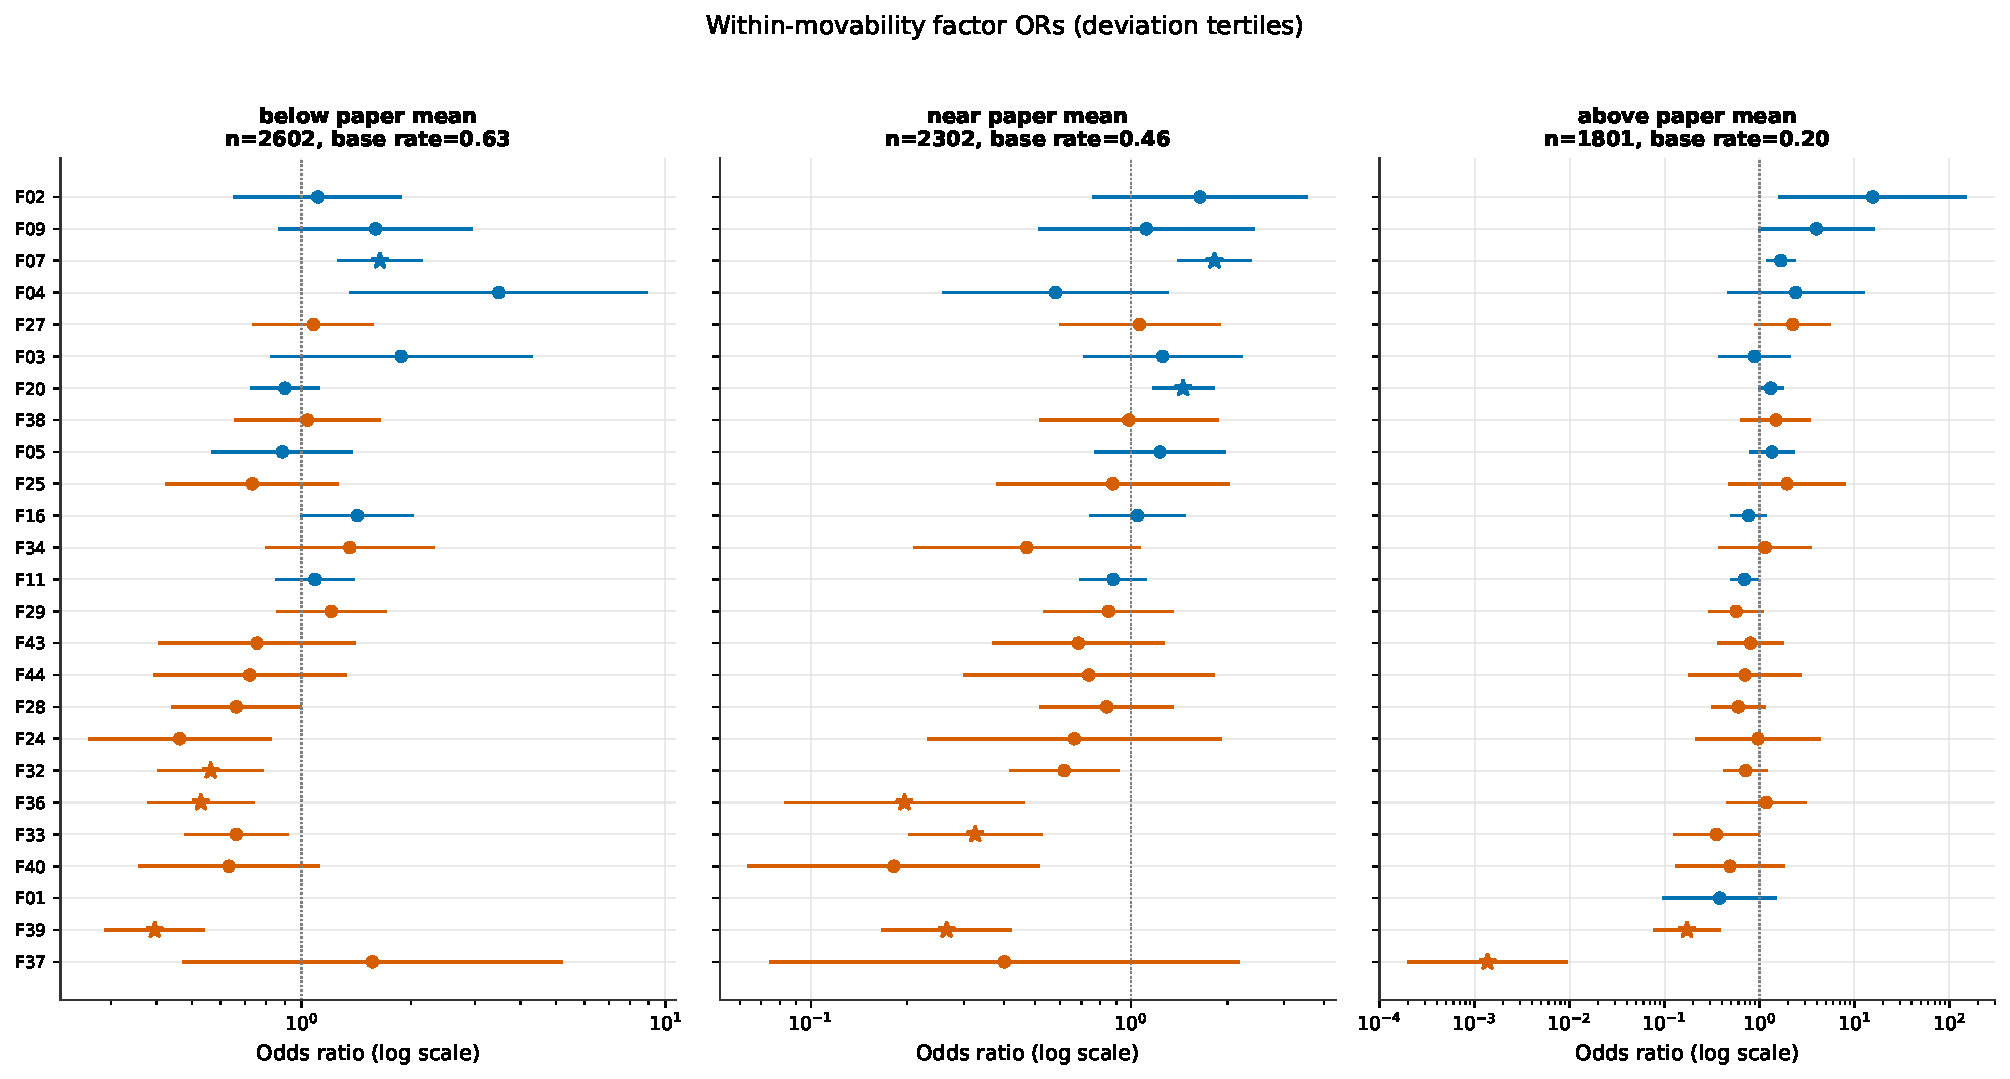
\includegraphics[width=0.85\linewidth]{forest_movability_strata.pdf}
  \caption{\textbf{Rebuttal-content factors within fixed movability strata.} Headline logistic refit on the cohort split by reviewer deviation from the paper-level initial mean: below ($n=2{,}602$), near ($n=2{,}302$), above ($n=1{,}801$). Markers: blue = positive, orange = negative; $\star$ = crosses Bonferroni $\alpha=0.05/44$ within the stratum. Y-axis: factors with $|\log\text{OR}|>0.3$ in any stratum.}
  \label{fig:movability-strata-app}
\end{figure}

\paragraph{Calibration on out-of-time data.} The same rebuttal-content logistic, refit on the year-$2024$ cohort only ($n = 5{,}710$) and evaluated on the year-$2025$ stratified slice ($n = 995$), produces predicted probabilities whose decile-binned means agree with the observed score-increase rate to within $\sim 0.05$ at the extremes (top decile predicted $0.94$ / observed $0.92$; bottom decile predicted $0.05$ / observed $0.15$) but with up to $\sim 0.20$ over-prediction in two middle deciles (predicted $\sim 0.65$ / observed $0.45$ and predicted $\sim 0.85$ / observed $0.75$). The 2025 slice is the stratified \Cref{res:taxonomy} (Test 1) sample, balanced across tier and verdict-group rather than naturally distributed. The bin-level observed rates are therefore noisy and cannot be reweighted to a population estimate without revisiting that stratification. Binned numbers: $\code{calibration\_temporal.csv}$.

\begin{figure}[!htb]
  \centering
  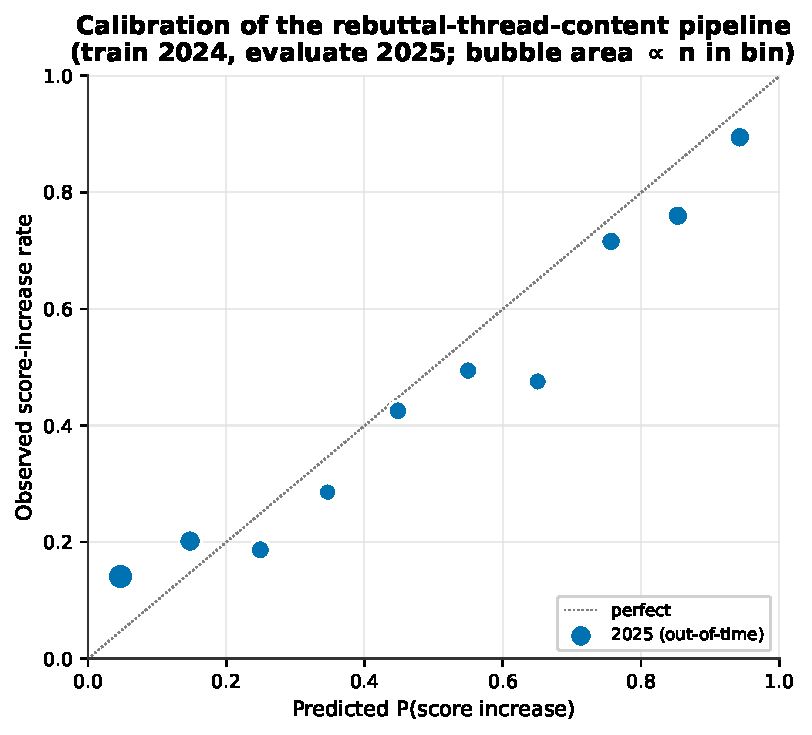
\includegraphics[width=0.55\linewidth]{calibration_temporal.pdf}
  \caption{\textbf{Out-of-time calibration of the rebuttal-content pipeline.} Train on ICLR 2024, predict on the ICLR 2025 stratified slice ($n=995$), bin into deciles by predicted probability. Bubble area $\propto$ bin sample size. Decile-level numbers in \Cref{app:horizons}.}
  \label{fig:calibration}
\end{figure}

\paragraph{Threshold metrics at $0.5$.} The headline cascade in \Cref{sec:rebuttal-impact} reports rank-based metrics ($\auc$, $\auprc$). For readers who want a directly interpretable success/no-success readout we additionally report accuracy, precision, recall, and $F_1$ at a fixed decision threshold of $p = 0.5$ for the rebuttal-content model (\Cref{tab:threshold-metrics}). On the temporal split (train year-$2024$, predict year-$2025$ stratified slice), the logistic reaches accuracy $72.6\%$ ($F_1 = 0.71$) against a $44.4\%$ base rate; under paper-clustered $\texttt{GroupKFold}(5)$ on the full $n = 6{,}705$ pool, accuracy reaches $77.1\%$ ($F_1 = 0.75$). The random forest underperforms the logistic on every threshold-based metric as well, consistent with the rank-based result. Threshold-$0.5$ numbers under-use the model's information: the calibration plot shows the rank ordering is reliable across all deciles while the absolute probability scale is reliable mainly at the extremes, so reporting at a single threshold is informative for context only. Source: $\code{threshold\_metrics\_draft.csv}$.

\begin{table}[h]
  \centering
  \caption{Threshold-$0.5$ classification metrics for the rebuttal-content logistic and random forest. Temporal split = train year-$2024$, predict year-$2025$ stratified slice; GroupKFold(5) = paper-clustered out-of-fold predictions on the combined $n = 6{,}705$ pool. Confusion-matrix cells: $tn$, $fp$, $fn$, $tp$.}
  \label{tab:threshold-metrics}
  \footnotesize
  \begin{tabular}{llrrrrrrrrrr}
    \toprule
    Split & Model & $n$ & base & acc. & prec. & recall & $F_1$ & $tn$ & $fp$ & $fn$ & $tp$ \\
    \midrule
    Temporal $2024 \to 2025$ & Logistic       & 995  & 0.444 & 0.726 & 0.666 & 0.767 & 0.713 & 383  & 170 & 103 & 339  \\
    Temporal $2024 \to 2025$ & Random forest  & 995  & 0.444 & 0.718 & 0.671 & 0.715 & 0.692 & 398  & 155 & 126 & 316  \\
    GroupKFold(5)            & Logistic       & 6705 & 0.456 & 0.771 & 0.739 & 0.770 & 0.754 & 2817 & 832 & 703 & 2353 \\
    GroupKFold(5)            & Random forest  & 6705 & 0.456 & 0.762 & 0.739 & 0.740 & 0.739 & 2849 & 800 & 795 & 2261 \\
    \bottomrule
  \end{tabular}
\end{table}

\paragraph{Scenario demonstrations.} For \Cref{tab:scenarios} we construct a "median-2024 author profile" by taking the median (continuous) or majority value (binary) for each feature on the year-2024 cohort, then read off the predicted probability under the listed factor-presence overrides. The scenario predictions are derived from the calibration-tested model (year-2024 fit), not the headline combined-data fit. Numbers: $\code{scenario\_predictions.csv}$.

\paragraph{Reproduction.}
\begin{itemize}[itemsep=0pt,topsep=2pt]
  \item Cascade-prediction (logistic + RF, three horizons, temporal + GroupKFold): $\code{src/analyze/exp34\_prediction\_horizons.py}$.
  \item Inferential analysis (paper-clustered logistic, marginal fits, ablations, recommendation gate, calibration, scenarios): $\code{src/analyze/exp33\_inference\_horizons.py}$.
  \item Row-level factor labels: $\code{data/results/32\_factor\_taxonomy/interaction\_factor\_labels\_\{2024,2025\}.csv}$.
  \item Cascade tables and figures: $\code{data/results/rebuttal\_rf\_prediction/}$.
  \item Inferential tables and figures: $\code{data/results/horizon\_inference/}$.
  \item Leakage tests: $\code{tests/test\_horizon\_leakage.py}$.
\end{itemize}

\subsection{Confidence-and-trigger analysis}\label{app:confidence-triggers}

To analyse what is associated with score revision, we focused on below-mean outlier reviewers (those who scored a paper lower than the co-reviewer average) and grouped them by confidence level and score-change outcome. We tested four families of potential triggers:
\begin{itemize}[itemsep=0pt,topsep=2pt]
  \item \textbf{Peer alignment.} Reviewer deviation from paper mean (z-score within the paper's review panel) and co-reviewer movement (share of co-reviewers who also increased their score after rebuttal).
  \item \textbf{Rebuttal effort.} Author reply length (in words and characters), number of author replies, and total thread message count.
  \item \textbf{Review characteristics.} Sub-scores (soundness, contribution, presentation), strength and weakness text lengths.
  \item \textbf{Engagement quality.} LLM-extracted engagement and actionability ratings from review text.
\end{itemize}

\paragraph{Operational definitions.}
\textit{Outlier} = z-score $\le -1.0$ within the paper's review panel (${\sim}15\%$ of reviews). \textit{Long rebuttal} = top quintile of reply length (more than \num{1574} words or \num{7870} characters). \textit{Peer-movement bucket} = share of co-reviewers who increased their score after rebuttal, binned into \{0, 1--25, 26--75, 76--100\}\%. \textit{Low confidence} = self-reported reviewer confidence $\le 3$ on the 5-point ICLR scale.

\paragraph{Statistical tests.}
Two-group comparisons used Mann-Whitney $U$ with rank-biserial correlation as effect size. Multi-group comparisons used Kruskal-Wallis with epsilon-squared, followed by pairwise Mann-Whitney with Bonferroni correction. Year-stratified replications (2024 vs.\ 2025) are reported alongside the combined estimates. Source figures: \code{data/results/confidence\_triggers/figures/}.

\subsection{Rebuttal content coding: 44-factor taxonomy with cross-model validation}\label{app:rebuttal-coding}

The factor taxonomy was induced and validated in three stages: induction with LLM-A (Claude), independent classification with LLM-B (Gemini Flash 3), and a held-out replication test on disjoint data. Two conditions were declared at the start of the analysis: (a) the factors reflect structure in the interaction text rather than patterns internal to LLM-A, and (b) the factor-outcome associations replicate beyond the induction sample.

\paragraph{Sample for taxonomy induction.}
From ICLR 2025 we drew \num{1000} reviewer-paper pairs stratified by reviewer initial rating (low 1--3, medium 5--6, high 8--10) crossed with rebuttal outcome (\code{increase} vs.\ \code{same\_decrease}), restricted to pairs with a non-empty author rebuttal thread. Each pair was serialised as a raw text thread containing the full original review (summary, strengths, weaknesses, questions), the full author rebuttal, and any reviewer follow-up comments, in chronological order. No structured Gemini-extracted fields (sentiment, tone, engagement-quality, score-change verdict outputs) were exposed to either LLM-A or LLM-B at any point in this analysis. The serialised threads are shipped at \code{data/results/factor\_validation/induction\_input\_1k\_threads\_iclr2025.json}. The high-increase cell is rare in ICLR 2025. We therefore used all 58 available pairs rather than subsample, which matches the strategy later applied to the ICLR 2024 hold-out. The remaining five cells were filled by random sampling.

\paragraph{Factor induction (LLM-A = Claude).}
In a single prompt we presented LLM-A with all six cells of the sample and instructed the model to perform the contrast within each tier (low-\code{increase} vs.\ low-\code{same\_decrease}, and analogously for medium and high). The within-tier framing preserves tier-specific patterns and prevents the model from collapsing the task into a single cross-tier contrast that could be dominated by score-level differences rather than rebuttal content. We repeated the procedure five times to attenuate run-to-run variability, then manually aggregated the extracted categories across runs and tiers, merging entries that were pure rephrasings or semantically close. The aggregation yielded 44 factors, each labelled with a declared polarity (positive or negative) from the pooled induction output.

\paragraph{Memory-control swaps.}
To rule out the hypothesis that LLM-A was retrieving canonical patterns from its prior rather than reading the interactions, we re-ran the induction under two manipulations. The first swapped the low-tier and high-tier interactions within the same prompt structure. The second silently swapped the \code{increase} and \code{same\_decrease} outcome labels on the same \num{1000} interactions, holding tier assignment fixed. In both cases the resulting factor content shifted with the presented inputs rather than tracking the labels, consistent with extraction from the interaction text. The outcome-label swap (the sharper of the two stress tests, since it operates on the axis the original induction used to discriminate) confirms that LLM-A continues to locate the same features on the same actual data even when the labels are flipped, and only the surface narrative re-frames around the new labels.

\paragraph{Classification protocol (LLM-B = Gemini Flash 3).}
A second, independent Gemini call classified each interaction against the fixed 44-factor list. The classifier saw the same raw thread text used at induction (no structured features), the 44-factor taxonomy with shuffled per-request factor identifiers, and the request to mark which factors were present. Classification was outcome-blinded: reviewer tier and rebuttal outcome were stripped from the prompt, factor identifiers were shuffled per request so that ordering could not cue the model, and the Gemini response schema constrained each returned \code{factor\_id} to the set F01--F44, blocking hallucinated categories. For every factor we computed an odds ratio comparing the \code{increase} and \code{same\_decrease} outcome groups, with a 95\% confidence interval, and a two-sided permutation test with 2000 permutations. Under each permutation the \code{increase} / \code{same\_decrease} labels are randomly reshuffled across interactions to simulate the null of no factor-outcome association, the odds ratio is recomputed, and the $p$-value is the fraction of shuffles whose $|\log \text{OR}|$ matches or exceeds the observed value (with add-one smoothing to keep $p > 0$). Significance is reported at the Bonferroni-corrected threshold $\alpha = 0.05 / 44 = 0.0011$. Choosing 2000 permutations gives a resolution floor of about $1/2001 \approx 0.0005$, just below the Bonferroni-corrected threshold.

\paragraph{Choice of multiple-testing correction.}
Bonferroni is the most stringent of the standard family-wise error-rate (FWER) controls and assumes nothing about test independence. We anchor on it because the held-out replication on a disjoint ICLR 2024 sample (Test 2) is itself a strong robustness check, and because surviving the strictest correction leaves least room for over-claiming. Two alternative corrections are reasonable, both more permissive (\Cref{tab:mtcorrection}). Holm-Bonferroni controls the same FWER as Bonferroni but is uniformly more powerful, and it yields 25 doubly-significant factors instead of 23. The Benjamini-Hochberg FDR rule controls the expected proportion of false positives among the rejected hypotheses (a weaker but often more appropriate guarantee for discovery-style analyses), and at $q = 0.05$ it yields 31 doubly-significant factors. Direction of effect agrees with the Bonferroni-anchored core under all three corrections, and the more permissive corrections add factors to the core rather than displace any of its members.

\begin{table}[htbp]
    \centering
    \caption{Sensitivity of the doubly-significant factor count to the multiple-testing correction. Bonferroni is the headline reported in \Cref{res:taxonomy}.}
    \label{tab:mtcorrection}
    \begin{tabular}{lccc}
    \toprule
    Correction & Test 1 & Test 2 & In both \\
    \midrule
    Uncorrected $p < 0.05$              & 32/44 & 43/44 & --- \\
    Bonferroni $\alpha = 0.05 / 44$    & 23/44 & 40/44 & \textbf{23/44} \\
    Holm-Bonferroni $\alpha = 0.05$    & 25/44 & 42/44 & 25/44 \\
    Benjamini-Hochberg $q = 0.05$      & 31/44 & 43/44 & 31/44 \\
    Benjamini-Hochberg $q = 0.10$      & 32/44 & 44/44 & 32/44 \\
    \bottomrule
    \end{tabular}
\end{table}

\paragraph{Tests.}
\textbf{Test 1 (operationalisability)} applies LLM-B to the same \num{1000} ICLR 2025 interactions used for induction, asking whether a second model can recover the induced factors from the same text. \textbf{Test 2 (discriminative validity)} applies the same protocol to the full classified ICLR 2024 cohort of \num{5730} interactions disjoint from the induction corpus, asking whether the factor-outcome associations replicate on fresh data. An earlier round of Test 2 was reported on a \num{952}-interaction stratified subsample of the same cohort (six-cell stratification by tier and verdict-group); the conclusions of that smaller test (43 of 44 declared polarities preserved, 16 of 44 doubly-Bonferroni-significant) hold under the present full-cohort version, with strict strengthening on every count. Source: \code{src/factor\_validation/expand\_test2\_full2024.py}; comparison CSV: \code{test2\_full2024\_comparison.csv}.

\paragraph{Cohort thinness and clustering.}
The classified ICLR 2024 cohort contains \num{5730} rebuttals across \num{3460} unique papers, an average of $1.66$ rebuttals per paper. This is a thinned slice of ICLR 2024's natural ${\sim}4$-reviewer paper structure, because not every reviewer wrote a rebuttal and not every (paper, reviewer) pair survived Gemini classification. The headline Test 2 permutation test uses naive (row-level) shuffling, matching the protocol used for the original Test 1 / Test 2 pair. As a robustness check we re-ran the expanded Test 2 with a within-paper block permutation that swaps outcome blocks at the paper level. The doubly-Bonferroni-significant count is unchanged at $23$ and per-factor $p$-values agree to within $0.005$. We do not lean on the block-permutation result as a paper-clustered correction in the body text, because the cohort thinness limits how much within-paper correlation our block test can detect, and we cannot rule out residual within-paper correlation in unobserved rebuttals or selection bias in which (paper, reviewer) pairs produced a classified rebuttal.

\paragraph{Results.}
The taxonomy shows the declared directional structure in both tests. In Test 1, 43 of 44 factors are more prevalent on the side of the \code{increase} versus \code{same\_decrease} contrast declared at induction (22 of 23 positive, 21 of 21 negative), and 23 of 44 survive the Bonferroni threshold. In Test 2, all 44 of 44 factors match their declared direction (23 of 23 positive, 21 of 21 negative), and 40 of 44 individually survive Bonferroni at the full-cohort sample size. The single Test 1 disagreement is F12 (proactive limitation acknowledgement) inverting polarity with OR = 0.90 [0.68, 1.19]; under the original \num{952}-interaction Test 2 subsample, F40 (marginal quantitative improvements) was the corresponding inversion at OR = 1.52 [0.76, 3.05], but it lands at OR = 0.36 [0.26, 0.51] in the full cohort, matching its declared negative polarity. Of the 44 factors, 23 cross Bonferroni in both tests (9 positive, 14 negative) and form the conservative core of the taxonomy. No factor crosses only in Test 1, and a further 17 cross only in Test 2 (the larger sample resolves several borderline factors that the in-sample run lacks power to detect). These are retained but reported as weaker evidence.

\begin{table}[htbp]
  \centering
  \caption{The 23 doubly-significant factors that anchor the taxonomy. ``Polarity'' is the direction declared at induction (LLM-A) and confirmed by both LLM-B tests at the Bonferroni-corrected threshold $\alpha = 0.05 / 44$.}
  \label{tab:taxonomy-core}
  \small
  \begin{tabular}{p{0.8cm} p{1.5cm} p{11cm}}
    \toprule
    \textbf{ID} & \textbf{Polarity} & \textbf{Label} \\
    \midrule
    F02 & positive & Non-defensive, respectful, collaborative tone. \\
    F04 & positive & Sincere engagement: detailed responses, length, added appendix content. \\
    F05 & positive & Methodological detail and reproducibility clarification. \\
    F06 & positive & Concrete empirical evidence tied to reviewer concerns. \\
    F07 & positive & Baseline completion / comparator strengthening. \\
    F13 & positive & Explicit manuscript revision signaling. \\
    F14 & positive & Supplementary material and new visual evidence. \\
    F21 & positive & Active dialogue and continued engagement. \\
    F22 & positive & Concrete revision commitments. \\
    \midrule
    F24 & negative & Defensive or dismissive tone. \\
    F25 & negative & Superficial or partial addressal of reviewer concerns. \\
    F27 & negative & Missing or insufficient baseline comparisons. \\
    F28 & negative & Lack of quantitative / empirical evidence in rebuttal. \\
    F29 & negative & No new requested experiments / analyses / ablations. \\
    F30 & negative & Vague future-oriented promises instead of concrete commitments. \\
    F31 & negative & Narrow or insufficient evaluation scope. \\
    F32 & negative & Incomplete empirical coverage even after rebuttal additions. \\
    F33 & negative & Unresolved quality-of-execution concerns that further experiments do not fix. \\
    F36 & negative & Weak novelty justification. \\
    F38 & negative & Section-referencing or paper-rephrasing instead of real clarification. \\
    F39 & negative & Inadequate explanation or persistent clarity issues. \\
    F42 & negative & Vague or insufficient technical explanation. \\
    F43 & negative & No explicit commitment to revise or improve the paper. \\
    \bottomrule
  \end{tabular}
\end{table}

Source: \code{data/results/factor\_validation/}. Induction prompt and classification prompt source files are referenced in \Cref{app:prompts}.

\subsection{Statistical framework}\label{app:stats}

We use non-parametric tests throughout, given the discrete and ordinal nature of reviewer ratings (six-point scale with uneven spacing \{1, 3, 5, 6, 8, 10\} for 2023 to 2025; see \Cref{app:dataset}). For two-group comparisons we use Mann-Whitney $U$ with rank-biserial correlation as effect size. For multi-group comparisons, Kruskal-Wallis with epsilon-squared. For correlations involving the score or confidence scales we report Spearman $\rho$ rather than Pearson $r$. Pearson's magnitude depends on the (arbitrary) numeric spacing of the scale, while Spearman, being rank-based, is invariant to it. For binary outcomes we use chi-squared or Fisher's exact tests with Cramer's V as effect size, and logistic regression with cluster-robust standard errors (statsmodels \code{cov\_type='cluster'}, \code{cov\_kwds=\{'groups': paper\_key\}}). For count data we use Mann-Whitney $U$ or Poisson / negative binomial regression.

Significance thresholds vary by analysis family because the families differ in test count and goal. We adopt the conventions in \Cref{tab:thresholds}, prioritising effect sizes over $p$-values, since with $n > \num{70000}$ even trivial differences reach conventional significance. All claims use predictive language (``associated with'', ``predicts'', ``co-occurs with''). We do not claim causation. Reviews within a paper are not independent (reviewers read the same manuscript and observe each other's scores during discussion), so all prediction models use \texttt{GroupKFold} by \code{paper\_key} and all regression coefficients use cluster-robust standard errors clustered on \code{paper\_key}.

\begin{table}[htbp]
  \centering
  \small
  \caption{Significance thresholds used in this paper, by analysis family.}
  \label{tab:thresholds}
  \begin{tabular}{p{6.5cm} p{7cm}}
  \toprule
  Analysis family & Threshold \\
  \midrule
  44-factor recommendation gate (\Cref{res:taxonomy,sec:horizons}) & Bonferroni $\alpha = 0.05/44 \approx 0.0011$ as the headline gate; BH $q = 0.05$ as a sensitivity (\Cref{tab:mtcorrection}) \\
  Asymmetric polarity screen (\Cref{sec:horizons}) & 95\% cluster-robust CI excludes $1$ in BOTH the marginal and polarity-isolated joint fits \\
  Structural/rebuttal-side covariates in the headline logistic (\Cref{sec:horizons}) & Conventional $p < 0.05$, reported with cluster-robust 95\% CIs and effect sizes \\
  Sign-test of declared polarity coherence (\Cref{app:horizons}) & Two-sided binomial, reported as exact $p$-value \\
  Descriptive non-parametric tests (\Cref{app:reviewer-agree,app:confidence-triggers}) & Mann-Whitney $U$, Kruskal-Wallis, Spearman $\rho$, Bonferroni-corrected within each family \\
  \bottomrule
  \end{tabular}
\end{table}

An inclusion funnel (\Cref{app:dataset}) documents the sample attrition at each analysis stage. Balance checks confirm that retained and excluded subsets do not differ systematically on initial score, confidence, or acceptance rate.

\subsection{Prompt availability and request examples}\label{app:prompts}

The exact prompts used by the three Gemini Flash 3 batch jobs (score decoder, score-change verdict classifier, and 44-factor classifier) and the Claude factor-induction prompt are reproduced verbatim in the companion code release at \code{src/prompts/} (\code{classification\_instruction.py}, \code{categorization\_prompt.py}) and \code{src/factor\_validation/} (induction and classification prompts), together with the JSON output schemas the calls were constrained to. A representative input/output pair for each Gemini prompt is bundled at \code{data/batches/batch\_input\_examples.json} so readers can inspect the exact request format without downloading the full batch corpus.

\subsection{Reproducibility}\label{app:repro}

\paragraph{Data and code availability.}
The full dataset is released on Hugging Face at \url{https://huggingface.co/datasets/MlouisBE/iclr-rebuttal-analysis}. It contains four artefact tiers: (i) the raw OpenReview JSON dumps for ICLR 2023--2026 ($\sim$3.0~GB) for full pipeline reproducibility; (ii) per-year analysis-ready parquet tables ($\sim$148~MB total: 14{,}339 reviews for 2023, 28{,}028 for 2024, 46{,}748 for 2025, 75{,}859 for 2026) joining review text, pre/post-rebuttal scores, Gemini-decoded scores, score-change verdicts, and the 44 factor indicators; (iii) consolidated Gemini batch outputs (per-year score-prediction files, per-year verdict files, and the factor-validation classifications with the full interaction text Gemini saw, paired with each $F_{01}\ldots F_{44}$ label); and (iv) all paper figures and tables.

\paragraph{License (per artefact tier).}
The release follows OpenReview's published terms~\cite{openreview-terms}, which the project applies separately to each underlying record type. Review comments, discussion messages, and configuration records (the bulk of the released text and our LLM-derived per-review labels) are redistributed under CC-BY-4.0, matching OpenReview's comment licence. Submission and venue metadata (\code{paper\_key}, \code{forum}, decision tier, timestamps) is redistributed under CC0 where OpenReview classifies it as such. Article and submission content (PDFs, abstracts, primary submission body) is \emph{not} redistributed in our release: only OpenReview-licensed comment text and our derived per-review tabular features ship in the parquet tables, and any reader who needs the underlying paper content must retrieve it directly from OpenReview under that paper's own licence field. Code (LaTeX source, analysis scripts, prompts, Makefile) is released under MIT in the companion \code{public\_release/} bundle. A representative input/output pair for each of the three Gemini prompts (score decoder, verdict classifier, factor classifier) is bundled at \code{data/batches/batch\_input\_examples.json} so readers can inspect the exact request format without downloading the full batch corpus.

Pipeline commands are wrapped in the \code{public\_release/Makefile} bundled with the submission. \code{make all} runs everything in order; \code{make sec31}, \code{make sec32}, \code{make sec33}, \code{make sec34} run the experiments behind each Results subsection; and \code{make methodology} runs the appendix experiments (reviewer agreement, regex-vs-Gemini benchmark, offset funnel, ground-truth profile). \code{make collect} and \code{make normalize} cover the data-preparation phases. \code{make help} lists all targets. The Python environment is captured in \code{requirements.txt}.

\paragraph{Random seeds.}
All sampling uses \code{random.seed(50)} (\code{src/core/sampling.py}: \code{get\_sampled\_indices(population, k, seed=50)}). The 1K validation sample described in \Cref{app:score-change} uses this seed.

\paragraph{Batch outputs and a data-integrity note.}
The full ICLR 2024 Gemini prediction file (\code{gemini\_3flash\_iclr2024\_full.json}) was originally produced by 25 chunked batch jobs. An early invocation of the \code{download-all} command before all chunks had completed left the assembled file with only 962 papers, corresponding to a 13.2\% review coverage. The file was subsequently rebuilt from all 25 chunks, yielding the correct 7,262 papers and 99.7\% review coverage. All numbers reported in the present paper use the rebuilt file.

\paragraph{Pipeline phases.}
Six numbered phases under \code{pipeline/} encode the dependency graph: collect ($\to$ raw JSON), normalise ($\to$ \code{data/processed/normalized/}), predict (Gemini batch submission and download), detect score changes (regex + Gemini verdict), analyse (the scripts under \code{src/analyze/}), and figures (the notebooks that produce the publication-ready PNG/PDF pairs in \code{data/results/figures/}). The \code{Makefile} encodes the dependencies between phases.

\end{document}
